\documentclass[]{article}
\usepackage{lmodern}
\usepackage{amssymb,amsmath}
\usepackage{ifxetex,ifluatex}
\usepackage{fixltx2e} % provides \textsubscript
\ifnum 0\ifxetex 1\fi\ifluatex 1\fi=0 % if pdftex
  \usepackage[T1]{fontenc}
  \usepackage[utf8]{inputenc}
\else % if luatex or xelatex
  \ifxetex
    \usepackage{mathspec}
  \else
    \usepackage{fontspec}
  \fi
  \defaultfontfeatures{Ligatures=TeX,Scale=MatchLowercase}
\fi
% use upquote if available, for straight quotes in verbatim environments
\IfFileExists{upquote.sty}{\usepackage{upquote}}{}
% use microtype if available
\IfFileExists{microtype.sty}{%
\usepackage{microtype}
\UseMicrotypeSet[protrusion]{basicmath} % disable protrusion for tt fonts
}{}
\usepackage[margin=1in]{geometry}
\usepackage{hyperref}
\hypersetup{unicode=true,
            pdftitle={ABAR: Chapter 3},
            pdfborder={0 0 0},
            breaklinks=true}
\urlstyle{same}  % don't use monospace font for urls
\usepackage{color}
\usepackage{fancyvrb}
\newcommand{\VerbBar}{|}
\newcommand{\VERB}{\Verb[commandchars=\\\{\}]}
\DefineVerbatimEnvironment{Highlighting}{Verbatim}{commandchars=\\\{\}}
% Add ',fontsize=\small' for more characters per line
\usepackage{framed}
\definecolor{shadecolor}{RGB}{248,248,248}
\newenvironment{Shaded}{\begin{snugshade}}{\end{snugshade}}
\newcommand{\KeywordTok}[1]{\textcolor[rgb]{0.13,0.29,0.53}{\textbf{#1}}}
\newcommand{\DataTypeTok}[1]{\textcolor[rgb]{0.13,0.29,0.53}{#1}}
\newcommand{\DecValTok}[1]{\textcolor[rgb]{0.00,0.00,0.81}{#1}}
\newcommand{\BaseNTok}[1]{\textcolor[rgb]{0.00,0.00,0.81}{#1}}
\newcommand{\FloatTok}[1]{\textcolor[rgb]{0.00,0.00,0.81}{#1}}
\newcommand{\ConstantTok}[1]{\textcolor[rgb]{0.00,0.00,0.00}{#1}}
\newcommand{\CharTok}[1]{\textcolor[rgb]{0.31,0.60,0.02}{#1}}
\newcommand{\SpecialCharTok}[1]{\textcolor[rgb]{0.00,0.00,0.00}{#1}}
\newcommand{\StringTok}[1]{\textcolor[rgb]{0.31,0.60,0.02}{#1}}
\newcommand{\VerbatimStringTok}[1]{\textcolor[rgb]{0.31,0.60,0.02}{#1}}
\newcommand{\SpecialStringTok}[1]{\textcolor[rgb]{0.31,0.60,0.02}{#1}}
\newcommand{\ImportTok}[1]{#1}
\newcommand{\CommentTok}[1]{\textcolor[rgb]{0.56,0.35,0.01}{\textit{#1}}}
\newcommand{\DocumentationTok}[1]{\textcolor[rgb]{0.56,0.35,0.01}{\textbf{\textit{#1}}}}
\newcommand{\AnnotationTok}[1]{\textcolor[rgb]{0.56,0.35,0.01}{\textbf{\textit{#1}}}}
\newcommand{\CommentVarTok}[1]{\textcolor[rgb]{0.56,0.35,0.01}{\textbf{\textit{#1}}}}
\newcommand{\OtherTok}[1]{\textcolor[rgb]{0.56,0.35,0.01}{#1}}
\newcommand{\FunctionTok}[1]{\textcolor[rgb]{0.00,0.00,0.00}{#1}}
\newcommand{\VariableTok}[1]{\textcolor[rgb]{0.00,0.00,0.00}{#1}}
\newcommand{\ControlFlowTok}[1]{\textcolor[rgb]{0.13,0.29,0.53}{\textbf{#1}}}
\newcommand{\OperatorTok}[1]{\textcolor[rgb]{0.81,0.36,0.00}{\textbf{#1}}}
\newcommand{\BuiltInTok}[1]{#1}
\newcommand{\ExtensionTok}[1]{#1}
\newcommand{\PreprocessorTok}[1]{\textcolor[rgb]{0.56,0.35,0.01}{\textit{#1}}}
\newcommand{\AttributeTok}[1]{\textcolor[rgb]{0.77,0.63,0.00}{#1}}
\newcommand{\RegionMarkerTok}[1]{#1}
\newcommand{\InformationTok}[1]{\textcolor[rgb]{0.56,0.35,0.01}{\textbf{\textit{#1}}}}
\newcommand{\WarningTok}[1]{\textcolor[rgb]{0.56,0.35,0.01}{\textbf{\textit{#1}}}}
\newcommand{\AlertTok}[1]{\textcolor[rgb]{0.94,0.16,0.16}{#1}}
\newcommand{\ErrorTok}[1]{\textcolor[rgb]{0.64,0.00,0.00}{\textbf{#1}}}
\newcommand{\NormalTok}[1]{#1}
\usepackage{graphicx,grffile}
\makeatletter
\def\maxwidth{\ifdim\Gin@nat@width>\linewidth\linewidth\else\Gin@nat@width\fi}
\def\maxheight{\ifdim\Gin@nat@height>\textheight\textheight\else\Gin@nat@height\fi}
\makeatother
% Scale images if necessary, so that they will not overflow the page
% margins by default, and it is still possible to overwrite the defaults
% using explicit options in \includegraphics[width, height, ...]{}
\setkeys{Gin}{width=\maxwidth,height=\maxheight,keepaspectratio}
\IfFileExists{parskip.sty}{%
\usepackage{parskip}
}{% else
\setlength{\parindent}{0pt}
\setlength{\parskip}{6pt plus 2pt minus 1pt}
}
\setlength{\emergencystretch}{3em}  % prevent overfull lines
\providecommand{\tightlist}{%
  \setlength{\itemsep}{0pt}\setlength{\parskip}{0pt}}
\setcounter{secnumdepth}{0}
% Redefines (sub)paragraphs to behave more like sections
\ifx\paragraph\undefined\else
\let\oldparagraph\paragraph
\renewcommand{\paragraph}[1]{\oldparagraph{#1}\mbox{}}
\fi
\ifx\subparagraph\undefined\else
\let\oldsubparagraph\subparagraph
\renewcommand{\subparagraph}[1]{\oldsubparagraph{#1}\mbox{}}
\fi

%%% Use protect on footnotes to avoid problems with footnotes in titles
\let\rmarkdownfootnote\footnote%
\def\footnote{\protect\rmarkdownfootnote}

%%% Change title format to be more compact
\usepackage{titling}

% Create subtitle command for use in maketitle
\newcommand{\subtitle}[1]{
  \posttitle{
    \begin{center}\large#1\end{center}
    }
}

\setlength{\droptitle}{-2em}
  \title{ABAR: Chapter 3}
  \pretitle{\vspace{\droptitle}\centering\huge}
  \posttitle{\par}
  \author{}
  \preauthor{}\postauthor{}
  \date{}
  \predate{}\postdate{}


\begin{document}
\maketitle

Data visualization is a critical tool in the data analysis process.
Visualization tasks can range from generating fundamental distribution
plots to understanding the interplay of complex influential variables in
machine learning algorithms. In this chapter we focus on the use of
visualization for initial \emph{data exploration}.

Visual data exploration is a mandatory intial step whether or not more
formal analysis follows. When combined with descriptive statistics
(Chapter\textasciitilde{}\ref{ch2:descriptive}), visualization provides
an effective way to identify summaries, structure, relationships,
differences, and abnormalities in the data. Often times no elaborate
analysis is necessary as all the important conclusions required for a
decision are evident from simple visual examination of the data
\textbf{(REF: Box and Hunter)}. Other times, data exploration will be
used to help guide the data cleaning, feature selection, and sampling
process.

Regardless, visual data exploration is about investigating the
characteristics of your data set. To do this, we typically create
numerous plots in an interactive fashion. This chapter will show you how
to create plots that answer some of the fundamental questions we
typically have of our data.

\section{Prerequisites}\label{prerequisites}

In this chapter we'll illustrate the key ideas by primarily focusing on
data from the \texttt{AmesHousing} package. We'll use \texttt{tidyverse}
to provide some basic data manipulation capabilities along with
\texttt{ggplot2} for plotting. We also demonstrate some useful functions
from a few other packages throughout the chapter.

\begin{Shaded}
\begin{Highlighting}[]
\KeywordTok{library}\NormalTok{(tidyverse)}
\KeywordTok{library}\NormalTok{(caret)}
\KeywordTok{library}\NormalTok{(GGally)}
\KeywordTok{library}\NormalTok{(treemap)}
\end{Highlighting}
\end{Shaded}

\begin{Shaded}
\begin{Highlighting}[]
\NormalTok{ames <-}\StringTok{ }\NormalTok{AmesHousing}\OperatorTok{::}\KeywordTok{make_ames}\NormalTok{()}
\end{Highlighting}
\end{Shaded}

\section{Univariate Distributions}\label{univariate-distributions}

Before moving on to more sophisticated visualizations that enable
multidimensional investigation, it is important to be able to understand
how an individual variable is distributed. Visually understanding the
distribution allows us to describe many features of a variable.

\subsection{Continuous Variables}\label{continuous-variables}

A variable is continuous if it can take any of an infinite set of
ordered values. There are several different plots that can effectively
communicate the different features of continuous variables. Features we
are generally interested in include:

\begin{itemize}
\tightlist
\item
  Measures of location
\item
  Measures of spread
\item
  Asymmetry
\item
  Outliers
\item
  Gaps
\end{itemize}

Histograms are often overlooked, yet they are a very efficient means for
communicating these features of continuous variables. Formulated by Karl
Pearson, histograms display numeric values on the x-axis where the
continuous variable is broken into intervals (aka bins) and the the
y-axis represents the frequency of observations that fall into that bin.
Histograms quickly signal what the most common observations are for the
variable being assessed (the higher the bar the more frequent those
values are observed in the data); they also signal the shape (spread and
symmetr) of your data by illustrating if the observed values cluster
towards one end or the other of the distribution.

To get a quick sense of how sales prices are distributed across the
2,930 properties in the \texttt{ames} data we can generate a simple
histogram by applying ggplot's \texttt{geom\_histogram}
function\footnote{We could also use \texttt{hist(ames\$Sale\_Price)} to
  produce a histogram with base R graphics.}. This histogram tells us
several important features about our variable:

\begin{itemize}
\tightlist
\item
  Measures of location: We can see the most common \texttt{Sale\_Price}
  is around the low \$100K.
\item
  Measures of spread: Our \texttt{Sale\_Price} ranges from near zero to
  over \$700K.
\item
  Asymmetry: \texttt{Sale\_Price} is skewed right (a common issue with
  financial data). Depending on the analytic technique we may want to
  apply later on this suggests we will likely need to transform this
  variable.
\item
  Outliers: It appears that there are some large values far from the
  other \texttt{Sale\_Price} values. Whether these are outliers in the
  mathematical sense or outliers to be concerned about is another issue
  but for now we at least know they exist.
\item
  Gaps: We see a gap exists between \texttt{Sale\_Price} values around
  \$650K and \$700K+.
\end{itemize}

\begin{Shaded}
\begin{Highlighting}[]
\KeywordTok{ggplot}\NormalTok{(ames, }\KeywordTok{aes}\NormalTok{(Sale_Price)) }\OperatorTok{+}
\StringTok{  }\KeywordTok{geom_histogram}\NormalTok{()}
\end{Highlighting}
\end{Shaded}

\begin{center}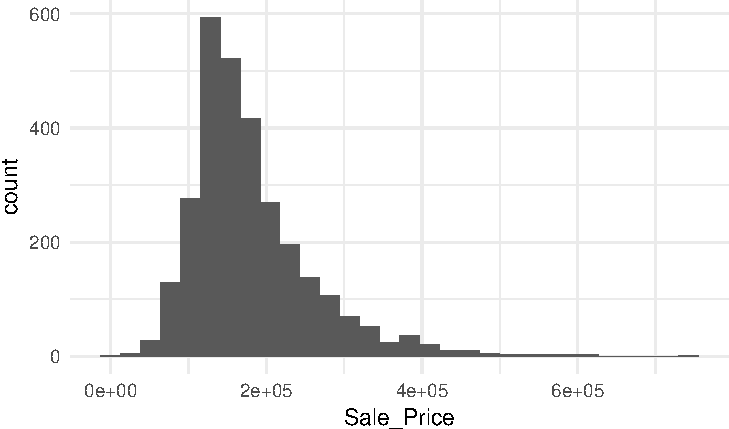
\includegraphics{Chapter_3_-_Visualization_files/figure-latex/hist1-1} \end{center}

By default, \texttt{geom\_histogram()} will divide your data into 30
equal bins or intervals. Since sales prices range from \$12,789 -
\$755,000, dividing this range into 30 equal bins means the bin width is
\$24,740. So the first bar will represent the frequency of
\texttt{Sale\_Price} values that range from about \$12,500 to about
\$37,500\footnote{These are approximates because the binning will round
  to whole numbers (12,800 rather than 12,370.)}, the second bar
represents the income range from about 37,500 to 62,300, and so on.

However, we can control this parameter by changing the bin width
argument in \texttt{geom\_histogram}. By changing the bin width when
doing exploratory analysis you can get a more detailed picture of the
relative densities of the distribution. For instance, in the default
histogram there was a bin of \$136,000 - \$161,000 values that had the
highest frequency but as the histograms that follow show, we can gather
more information as we adjust the binning.

\begin{Shaded}
\begin{Highlighting}[]

\NormalTok{p1 <-}\StringTok{ }\KeywordTok{ggplot}\NormalTok{(ames, }\KeywordTok{aes}\NormalTok{(Sale_Price)) }\OperatorTok{+}
\StringTok{  }\KeywordTok{geom_histogram}\NormalTok{(}\DataTypeTok{binwidth =} \DecValTok{100000}\NormalTok{) }\OperatorTok{+}
\StringTok{  }\KeywordTok{ggtitle}\NormalTok{(}\StringTok{"Bin width = $100,000"}\NormalTok{)}

\NormalTok{p2 <-}\StringTok{ }\KeywordTok{ggplot}\NormalTok{(ames, }\KeywordTok{aes}\NormalTok{(Sale_Price)) }\OperatorTok{+}
\StringTok{  }\KeywordTok{geom_histogram}\NormalTok{(}\DataTypeTok{binwidth =} \DecValTok{50000}\NormalTok{) }\OperatorTok{+}
\StringTok{  }\KeywordTok{ggtitle}\NormalTok{(}\StringTok{"Bin width = $50,000"}\NormalTok{)}

\NormalTok{p3 <-}\StringTok{ }\KeywordTok{ggplot}\NormalTok{(ames, }\KeywordTok{aes}\NormalTok{(Sale_Price)) }\OperatorTok{+}
\StringTok{  }\KeywordTok{geom_histogram}\NormalTok{(}\DataTypeTok{binwidth =} \DecValTok{5000}\NormalTok{) }\OperatorTok{+}
\StringTok{  }\KeywordTok{ggtitle}\NormalTok{(}\StringTok{"Bin width = $5,000"}\NormalTok{)}

\NormalTok{p4 <-}\StringTok{ }\KeywordTok{ggplot}\NormalTok{(ames, }\KeywordTok{aes}\NormalTok{(Sale_Price)) }\OperatorTok{+}
\StringTok{  }\KeywordTok{geom_histogram}\NormalTok{(}\DataTypeTok{binwidth =} \DecValTok{1000}\NormalTok{) }\OperatorTok{+}
\StringTok{  }\KeywordTok{ggtitle}\NormalTok{(}\StringTok{"Bin width = $1,000"}\NormalTok{)}

\NormalTok{gridExtra}\OperatorTok{::}\KeywordTok{grid.arrange}\NormalTok{(p1, p2, p3, p4, }\DataTypeTok{ncol =} \DecValTok{2}\NormalTok{)}
\end{Highlighting}
\end{Shaded}

\begin{center}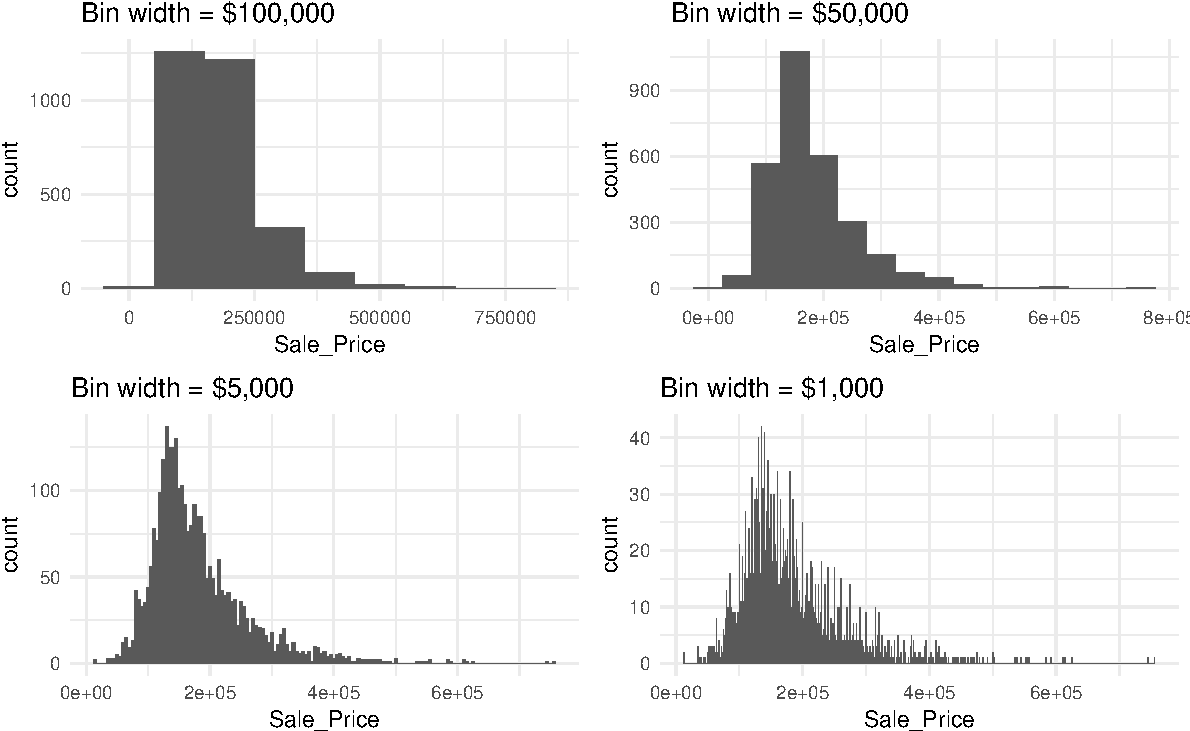
\includegraphics{Chapter_3_-_Visualization_files/figure-latex/hist2-1} \end{center}

Overall, the histograms consistently show the most common income level
to be right around \$130,000. We can also find the most frequent bin by
combining \texttt{ggplot2::cut\_width} (\texttt{ggplot2::cut\_interval}
and \texttt{ggplot2::cut\_number} are additional options) with
\texttt{dplyr::count}. We see that the most frequent bin when using
increments of \$5,000 is \$128,000 - \$132,000.

\begin{Shaded}
\begin{Highlighting}[]
\NormalTok{ames }\OperatorTok
\StringTok{  }\KeywordTok{count}\NormalTok{(}\KeywordTok{cut_width}\NormalTok{(Sale_Price, }\DataTypeTok{width =} \DecValTok{5000}\NormalTok{)) }\OperatorTok
\StringTok{  }\KeywordTok{arrange}\NormalTok{(}\KeywordTok{desc}\NormalTok{(n))}
\NormalTok{## # A tibble: 106 x 2}
\NormalTok{##    `cut_width(Sale_Price, width = 5000)`     n}
\NormalTok{##    <fctr>                                <int>}
\NormalTok{##  1 (1.28e+05,1.32e+05]                     137}
\NormalTok{##  2 (1.42e+05,1.48e+05]                     130}
\NormalTok{##  3 (1.32e+05,1.38e+05]                     125}
\NormalTok{##  4 (1.38e+05,1.42e+05]                     125}
\NormalTok{##  5 (1.22e+05,1.28e+05]                     118}
\NormalTok{##  6 (1.52e+05,1.58e+05]                     103}
\NormalTok{##  7 (1.48e+05,1.52e+05]                     101}
\NormalTok{##  8 (1.18e+05,1.22e+05]                      99}
\NormalTok{##  9 (1.58e+05,1.62e+05]                      92}
\NormalTok{## 10 (1.72e+05,1.78e+05]                      92}
\NormalTok{## # ... with 96 more rows}
\end{Highlighting}
\end{Shaded}

Our histogram with \texttt{binwidth\ =\ 1000} also shows us that there
are spikes at specific intervals. This is likely due to home sale prices
usually occuring around increments of \$5,000. In addition to our
primary central tendency (bins with most frequency), we also get a
clearer picture of the spread of our variable and its skewness. This
suggests there may be a concern with our variable meeting assumptions of
normality. If we were to apply an analytic technique that is sensitive
to normality assumptions we would likely need to transform our variable.

We can assess the applicability of a log transformation by adding
\texttt{scale\_x\_log()} to our ggplot visual\footnote{Two things to
  note here. 1. If you want to change the binwidth you either need to
  feed a log tranformed number to binwidth or, as I did, increase the
  bins by using \texttt{bins\ =\ 100}. 2. If you have values of zero in
  your variable try `scale\_x\_continuous(trans = ``log1p''), which adds
  1 prior to the log transformation.}. This log transformed histogram
provides a few new insights:

\begin{enumerate}
\def\labelenumi{\arabic{enumi}.}
\tightlist
\item
  There is a slight multimodal effect at the top of the distribution
  suggesting that houses selling in the \$150-170K range are not as
  common as those selling just below and above that price range.
\item
  It appears the log transformation helps our variable meet normality
  assumptions. More on this in a second.
\item
  It appears there is a new potential outlier that we did not see
  earlier. There is at least one observation where the
  \texttt{Sale\_Price} is near zero. In fact, further investigation
  identifies two observations, one with a \texttt{Sale\_Price} of
  \$12,789 and another at \$13,100.
\end{enumerate}

\begin{Shaded}
\begin{Highlighting}[]
\KeywordTok{ggplot}\NormalTok{(ames, }\KeywordTok{aes}\NormalTok{(Sale_Price)) }\OperatorTok{+}
\StringTok{  }\KeywordTok{geom_histogram}\NormalTok{(}\DataTypeTok{bins =} \DecValTok{100}\NormalTok{) }\OperatorTok{+}
\StringTok{  }\KeywordTok{geom_vline}\NormalTok{(}\DataTypeTok{xintercept =} \KeywordTok{c}\NormalTok{(}\DecValTok{150000}\NormalTok{, }\DecValTok{170000}\NormalTok{), }\DataTypeTok{color =} \StringTok{"red"}\NormalTok{, }\DataTypeTok{lty =} \StringTok{"dashed"}\NormalTok{) }\OperatorTok{+}
\StringTok{  }\KeywordTok{scale_x_log10}\NormalTok{(}
    \DataTypeTok{labels =}\NormalTok{ scales}\OperatorTok{::}\NormalTok{dollar, }
    \DataTypeTok{breaks =} \KeywordTok{c}\NormalTok{(}\DecValTok{50000}\NormalTok{, }\DecValTok{125000}\NormalTok{, }\DecValTok{300000}\NormalTok{)}
\NormalTok{    )}
\end{Highlighting}
\end{Shaded}

\begin{center}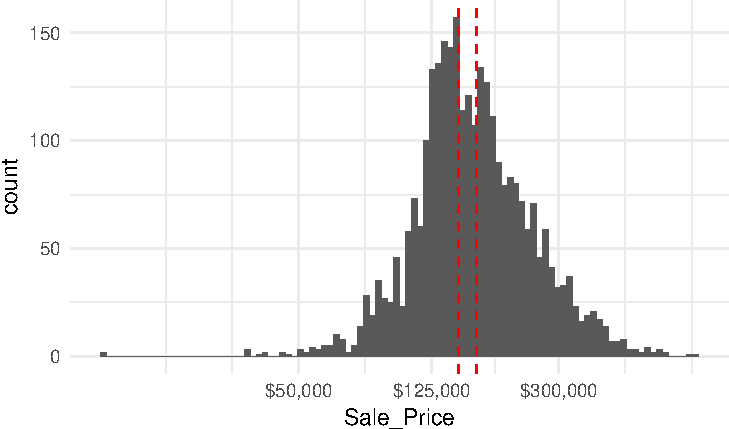
\includegraphics{Chapter_3_-_Visualization_files/figure-latex/logtrans-1} \end{center}

Let's take a closer look at the second two insights. First, we'll
consider the issue of normality.

If you really want to look at normality, then Q-Q plots are a great
visual to assess (Fig xx). This graph plots the cumulative values we
have in our data against the cumulative probability of a particular
distribution (the default is a normal distribution). In essence, this
plot compares the actual value against the expected value that the score
should have in a normal distribution. If the data are normally
distributed the plot will display a straight (or nearly straight) line.
If the data deviates from normality then the line will display strong
curvature or ``snaking.'' These plots illustrate how much the
untransformed variable deviates from normality whereas the log
transformed values align much closer to a normal distribution.

\begin{Shaded}
\begin{Highlighting}[]
\KeywordTok{par}\NormalTok{(}\DataTypeTok{mfrow =} \KeywordTok{c}\NormalTok{(}\DecValTok{1}\NormalTok{, }\DecValTok{2}\NormalTok{))}

\CommentTok{# non-log transformed}
\KeywordTok{qqnorm}\NormalTok{(ames}\OperatorTok{$}\NormalTok{Sale_Price, }\DataTypeTok{main =} \StringTok{"Untransformed}\CharTok{\textbackslash{}n}\StringTok{Normal Q-Q Plot"}\NormalTok{)}
\KeywordTok{qqline}\NormalTok{(ames}\OperatorTok{$}\NormalTok{Sale_Price)}

\CommentTok{# log transformed}
\KeywordTok{qqnorm}\NormalTok{(}\KeywordTok{log}\NormalTok{(ames}\OperatorTok{$}\NormalTok{Sale_Price), }\DataTypeTok{main =} \StringTok{"Log Transformed}\CharTok{\textbackslash{}n}\StringTok{Normal Q-Q Plot"}\NormalTok{)}
\KeywordTok{qqline}\NormalTok{(}\KeywordTok{log}\NormalTok{(ames}\OperatorTok{$}\NormalTok{Sale_Price))}
\end{Highlighting}
\end{Shaded}

\begin{center}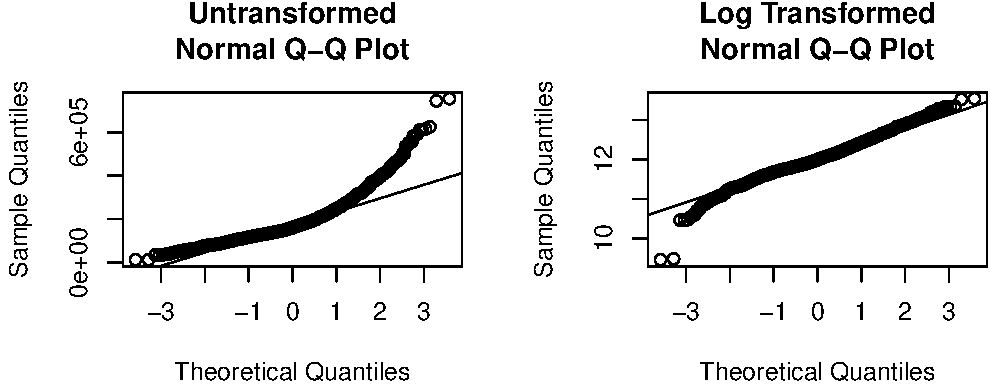
\includegraphics{Chapter_3_-_Visualization_files/figure-latex/qqplot-1} \end{center}

I also mentioned how we obtained a new insight regarding a new potential
outlier that we did not see earlier. So far our histogram identified
potential outliers at the lower end and upper end of the sale price
spectrum. Unfortunately histograms are not very good at delineating
outliers. Rather, we can use a boxplot which does a better job
identifying specific outliers.

Boxplots are an alternative way to illustrate the distribution of a
variable and is a concise way to illustrate the standard quantiles and
outliers of data. As Figure XX indicates, the box itself extends, left
to right, from the 1st quartile to the 3rd quartile. This means that it
contains the middle half of the data. The line inside the box is
positioned at the median. The lines (whiskers) coming out either side of
the box extend to 1.5 interquartile ranges (IQRs) from the quartiles.
These generally include most of the data outside the box. More distant
values, called outliers, are denoted separately by individual points.
Now we have a more analytically specific approach to identifying
outliers.

There are two efficient graphs to get an indication of potential
outliers in our data. The classic boxplot on the left will identify
points beyond the whiskers which are beyond \(1.5*IQR\) from the first
and third quantile. This illustrates there are several additional
observations that we may need to assess as outliers that were not
evident in our histogram. However, when looking at a boxplot we lose
insight into the shape of the distribution. A violin plot on the right
provides us a similar chart as the boxplot but we lose insight into the
quantiles of our data and outliers are not plotted (hence the reason I
plot \texttt{geom\_point} prior to \texttt{geom\_violin}). Violin plots
will come in handy later when we start to visualize multiple
distributions along side each other.

\begin{Shaded}
\begin{Highlighting}[]
\NormalTok{p1 <-}\StringTok{ }\KeywordTok{ggplot}\NormalTok{(ames, }\KeywordTok{aes}\NormalTok{(}\StringTok{"var"}\NormalTok{, Sale_Price)) }\OperatorTok{+}
\StringTok{  }\KeywordTok{geom_boxplot}\NormalTok{(}\DataTypeTok{outlier.alpha =}\NormalTok{ .}\DecValTok{25}\NormalTok{) }\OperatorTok{+}
\StringTok{  }\KeywordTok{scale_y_log10}\NormalTok{(}
    \DataTypeTok{labels =}\NormalTok{ scales}\OperatorTok{::}\NormalTok{dollar, }
    \DataTypeTok{breaks =} \KeywordTok{quantile}\NormalTok{(ames}\OperatorTok{$}\NormalTok{Sale_Price)}
\NormalTok{  )}

\NormalTok{p2 <-}\StringTok{ }\KeywordTok{ggplot}\NormalTok{(ames, }\KeywordTok{aes}\NormalTok{(}\StringTok{"var"}\NormalTok{, Sale_Price)) }\OperatorTok{+}
\StringTok{  }\KeywordTok{geom_point}\NormalTok{() }\OperatorTok{+}
\StringTok{  }\KeywordTok{geom_violin}\NormalTok{() }\OperatorTok{+}
\StringTok{  }\KeywordTok{scale_y_log10}\NormalTok{(}
    \DataTypeTok{labels =}\NormalTok{ scales}\OperatorTok{::}\NormalTok{dollar, }
    \DataTypeTok{breaks =} \KeywordTok{quantile}\NormalTok{(ames}\OperatorTok{$}\NormalTok{Sale_Price)}
\NormalTok{  )}

\NormalTok{gridExtra}\OperatorTok{::}\KeywordTok{grid.arrange}\NormalTok{(p1, p2, }\DataTypeTok{ncol =} \DecValTok{2}\NormalTok{)}
\end{Highlighting}
\end{Shaded}

\begin{center}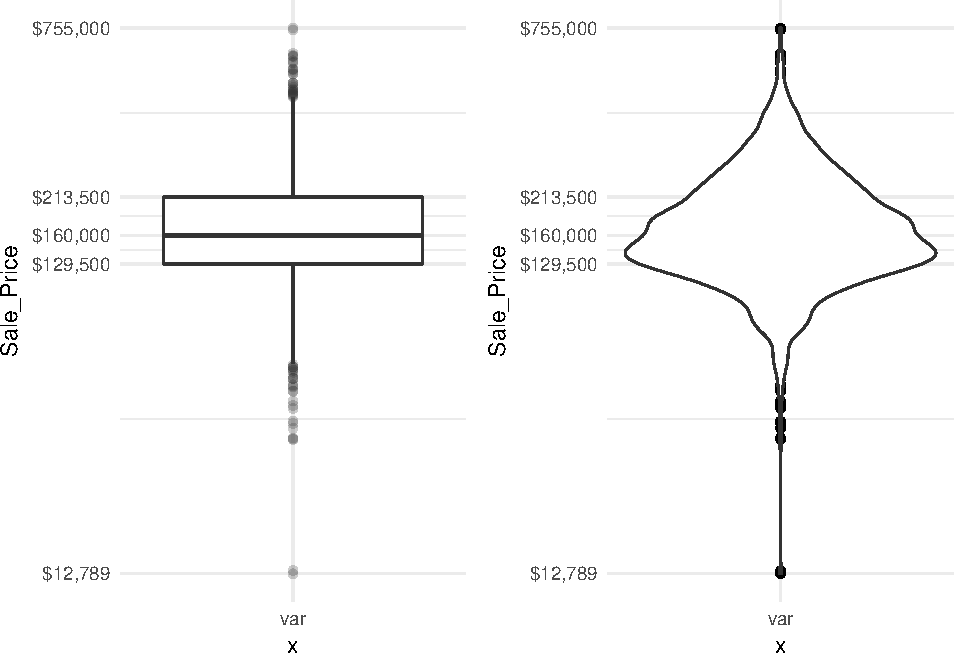
\includegraphics{Chapter_3_-_Visualization_files/figure-latex/boxplot-1} \end{center}

The boxplot starts to answer the question of what potential outliers
exist in our data. Outliers in data can distort predictions and affect
their accuracy. Consequently, its important to understand if outliers
are present and, if so, which observations are considered outliers.
Boxplots provide a visual assessment of potential outliers while the
\texttt{outliers} package provides a number of useful functions to
systematically extract these outliers. The most useful function is the
\texttt{scores} function, which computes normal, t, chi-squared, IQR and
MAD scores of the given data which you can use to find observation(s)
that lie beyond a given value.

Here, I use the \texttt{outliers::score} function to extract those
observations beyond the whiskers in our boxplot and then use a
stem-and-leaf plot to assess them. A stem-and-leaf plot is a special
table where each data value is split into a ``stem'' (the first digit or
digits) and a ``leaf'' (usually the second digit). Since the decimal
point is located 5 digits to the right of the ``\textbar{}''" the last
stem of ``7'' and and first leaf of ``5'' means an outlier exists at
around \$750,000. The last stem of ``7'' and and second leaf of ``6''
means an outlier exists at around \$760,000. This is a concise way to
see approximately where our outliers are. In fact, I can now see that I
have 28 lower end outliers ranging from \$10,000-\$60,000 and 32 upper
end outliers ranging from \$450,000-\$760,000.

\begin{Shaded}
\begin{Highlighting}[]
\NormalTok{outliers <-}\StringTok{ }\NormalTok{outliers}\OperatorTok{::}\KeywordTok{scores}\NormalTok{(}\KeywordTok{log}\NormalTok{(ames}\OperatorTok{$}\NormalTok{Sale_Price), }\DataTypeTok{type =} \StringTok{"iqr"}\NormalTok{, }\DataTypeTok{lim =} \FloatTok{1.5}\NormalTok{)}
\KeywordTok{stem}\NormalTok{(ames}\OperatorTok{$}\NormalTok{Sale_Price[outliers])}
\NormalTok{## }
\NormalTok{##   The decimal point is 5 digit(s) to the right of the |}
\NormalTok{## }
\NormalTok{##   0 | 1134444445555555666666666666}
\NormalTok{##   1 | }
\NormalTok{##   2 | }
\NormalTok{##   3 | }
\NormalTok{##   4 | 56666777788899}
\NormalTok{##   5 | 000445566889}
\NormalTok{##   6 | 1123}
\NormalTok{##   7 | 56}
\end{Highlighting}
\end{Shaded}

Another useful plot for univariate assessment includes the
\emph{smoothed} histogram in which a non-parametric approach is used to
estimate the density function. Displaying in density form just means the
y-axis is now in a probability scale where the proportion of the given
value (or bin of values) to the overall population is displayed. In
essence, the y-axis tells you the estimated probability of the x-axis
value occurring. This results in a \emph{smoothed} curve known as the
density plot that allows us visualize the distribution. Since the focus
of a density plot is to view the overall distribution rather than
individual bin observations we lose insight into how many observations
occur at certain x values. Consequently, it can be helpful to use
\texttt{geom\_rug} with \texttt{geom\_density} to highlight where
clusters, outliers, and gaps of observations are occuring.

\begin{Shaded}
\begin{Highlighting}[]
\NormalTok{p1 <-}\StringTok{ }\KeywordTok{ggplot}\NormalTok{(ames, }\KeywordTok{aes}\NormalTok{(Sale_Price)) }\OperatorTok{+}
\StringTok{  }\KeywordTok{geom_density}\NormalTok{()}

\NormalTok{p2 <-}\StringTok{ }\KeywordTok{ggplot}\NormalTok{(ames, }\KeywordTok{aes}\NormalTok{(Sale_Price)) }\OperatorTok{+}
\StringTok{  }\KeywordTok{geom_density}\NormalTok{() }\OperatorTok{+}
\StringTok{  }\KeywordTok{geom_rug}\NormalTok{()}

\NormalTok{gridExtra}\OperatorTok{::}\KeywordTok{grid.arrange}\NormalTok{(p1, p2, }\DataTypeTok{nrow =} \DecValTok{1}\NormalTok{)}
\end{Highlighting}
\end{Shaded}

\begin{center}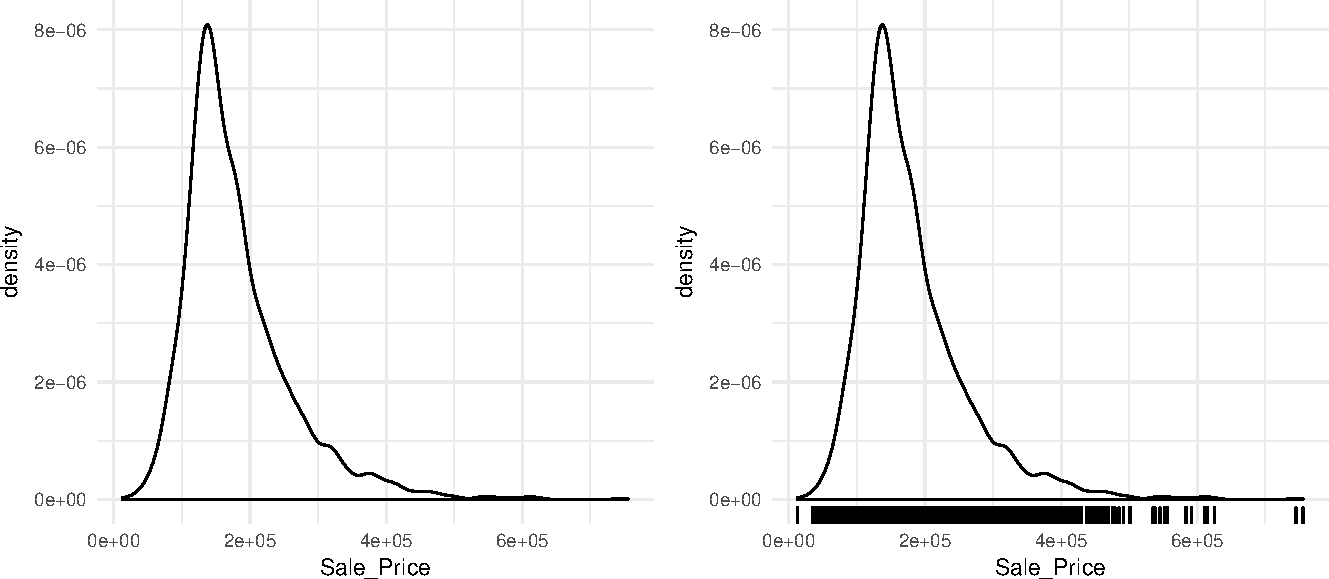
\includegraphics{Chapter_3_-_Visualization_files/figure-latex/density-1} \end{center}

Often you will see density plots layered onto histograms. To layer the
density plot onto the histogram we need to first draw the histogram but
tell ggplot to have the y-axis in density form rather than count. You
can then add the \texttt{geom\_density} function to add the density plot
on top.

\begin{Shaded}
\begin{Highlighting}[]
\KeywordTok{ggplot}\NormalTok{(ames, }\KeywordTok{aes}\NormalTok{(Sale_Price)) }\OperatorTok{+}
\StringTok{  }\KeywordTok{geom_histogram}\NormalTok{(}\KeywordTok{aes}\NormalTok{(}\DataTypeTok{y =}\NormalTok{ ..density..),}
                 \DataTypeTok{binwidth =} \DecValTok{5000}\NormalTok{, }\DataTypeTok{color =} \StringTok{"grey30"}\NormalTok{, }\DataTypeTok{fill =} \StringTok{"white"}\NormalTok{) }\OperatorTok{+}
\StringTok{  }\KeywordTok{geom_density}\NormalTok{(}\DataTypeTok{alpha =}\NormalTok{ .}\DecValTok{2}\NormalTok{, }\DataTypeTok{fill =} \StringTok{"antiquewhite3"}\NormalTok{)}
\end{Highlighting}
\end{Shaded}

\begin{center}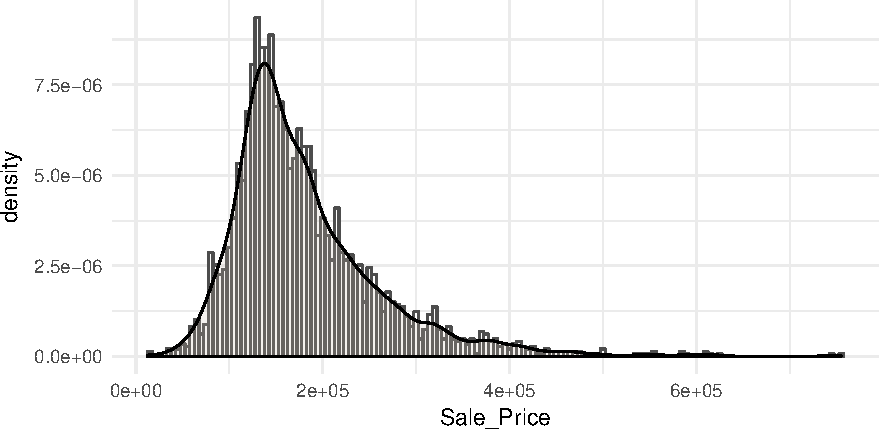
\includegraphics{Chapter_3_-_Visualization_files/figure-latex/density2-1} \end{center}

You may also be interested to see if there are any systematic groupings
with how the data is structured. For example, using base R's
\texttt{plot} function with just the \texttt{Sale\_Price} will plot the
sale price versus the index (row) number of each observation. In the
plot below we see a pattern which indicates that groupings of homes with
high versus lower sale prices are concentrated together throughout the
data set.

\begin{Shaded}
\begin{Highlighting}[]
\KeywordTok{plot}\NormalTok{(ames}\OperatorTok{$}\NormalTok{Sale_Price)}
\end{Highlighting}
\end{Shaded}

\begin{center}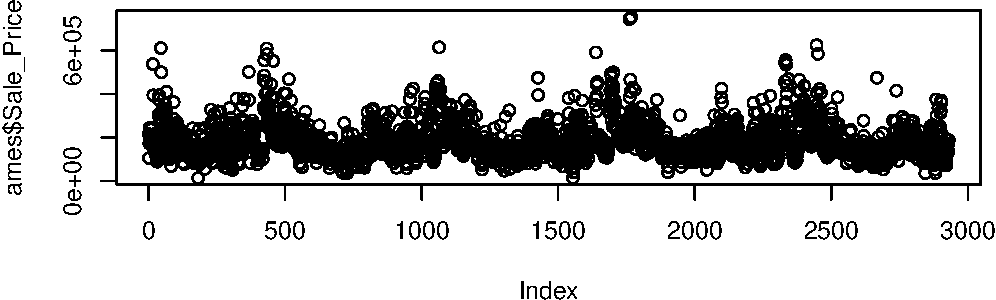
\includegraphics{Chapter_3_-_Visualization_files/figure-latex/indexplot-1} \end{center}

There are also a couple plots that can come in handy when dealing with
smaller data sets. For example, the dotplot below provides more clarity
than the histogram for viewing the distribution of \texttt{mpg} in the
built-in \texttt{mtcars} dataset with only 32 observations. An
alternative to this would be using a strip chart (see
\texttt{stripchart}).

\begin{Shaded}
\begin{Highlighting}[]
\NormalTok{p1 <-}\StringTok{ }\KeywordTok{ggplot}\NormalTok{(mtcars, }\KeywordTok{aes}\NormalTok{(}\DataTypeTok{x =}\NormalTok{ mpg)) }\OperatorTok{+}
\StringTok{  }\KeywordTok{geom_dotplot}\NormalTok{(}\DataTypeTok{method =} \StringTok{"histodot"}\NormalTok{, }\DataTypeTok{binwidth =} \DecValTok{1}\NormalTok{) }\OperatorTok{+}
\StringTok{  }\KeywordTok{ggtitle}\NormalTok{(}\StringTok{"dotplot"}\NormalTok{)}

\NormalTok{p2 <-}\StringTok{ }\KeywordTok{ggplot}\NormalTok{(mtcars, }\KeywordTok{aes}\NormalTok{(}\DataTypeTok{x =}\NormalTok{ mpg)) }\OperatorTok{+}
\StringTok{  }\KeywordTok{geom_histogram}\NormalTok{(}\DataTypeTok{binwidth =} \DecValTok{1}\NormalTok{) }\OperatorTok{+}
\StringTok{  }\KeywordTok{ggtitle}\NormalTok{(}\StringTok{"histogram"}\NormalTok{)}

\NormalTok{gridExtra}\OperatorTok{::}\KeywordTok{grid.arrange}\NormalTok{(p1, p2, }\DataTypeTok{nrow =} \DecValTok{1}\NormalTok{)}
\end{Highlighting}
\end{Shaded}

\begin{center}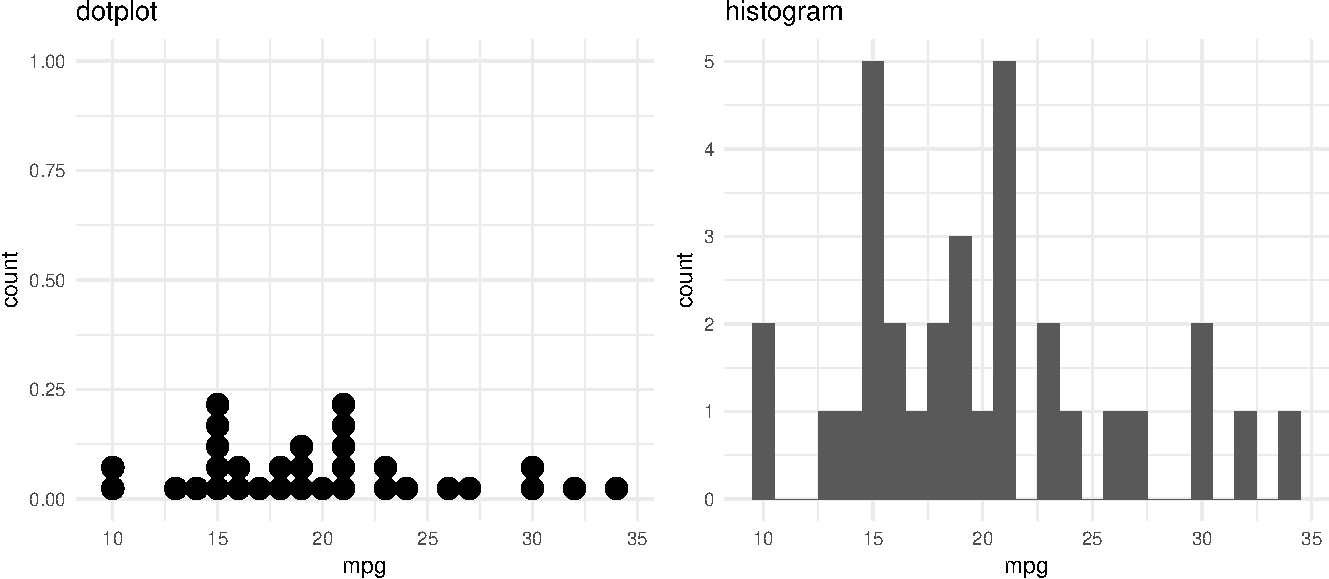
\includegraphics{Chapter_3_-_Visualization_files/figure-latex/dotplot-1} \end{center}

As demonstrated, several plots exist for examining univariate continuous
variables. Several exampes were provided here but still more exist
(i.e.~frequency polygon, beanplot, shifted histograms). There is some
general advice to follow such as histograms being poor for small data
sets, dotplots being poor for large data sets, histograms being poor for
identifying outlier cut-offs, boxplots being good for outliers but
obscuring multimodality. Conseqently, it is important to draw a variety
of plots. Moreover, it is important to adjust parameters within plots
(i.e.~binwidth, axis transformation for skewed data) to get a
comprehensive picture of the variable of concern.

\subsection{Categorical Variables}\label{categorical-variables}

A categorical variable is a variable that can take on one of a limited,
and usually fixed, number of possible values, assigning each individual
or other unit of observation to a particular group or nominal category
on the basis of some qualitative property (i.e.~gender, grade,
manufacturer). There are a few different plots that can effectively
communicate features of categorical variables. Features we are generally
interested in include:

\begin{itemize}
\tightlist
\item
  Count of each category
\item
  Proportion of each category
\item
  Imbalanced categories
\item
  Mislabeled categories
\end{itemize}

Bar charts are one of the most commonly used data visualizations for
categorical variables. Bar charts display the levels of a categorical
variable of interest (typically) along the x-axis and the length of the
bar illustrates the value along the y-axis. Consequently, the length of
the bar is the primary visual cue in a bar chart and in a univariate
visualization this length represents counts of cases in that particular
level.

If we look at the general zoning classification for each property sold
in our \texttt{ames} dataset we see that the majority of all properties
fall within one category. Here, \texttt{geom\_bar} simply counts up all
observations for each zoning level.

\begin{Shaded}
\begin{Highlighting}[]
\KeywordTok{ggplot}\NormalTok{(ames, }\KeywordTok{aes}\NormalTok{(MS_Zoning)) }\OperatorTok{+}
\StringTok{  }\KeywordTok{geom_bar}\NormalTok{()}
\end{Highlighting}
\end{Shaded}

\begin{center}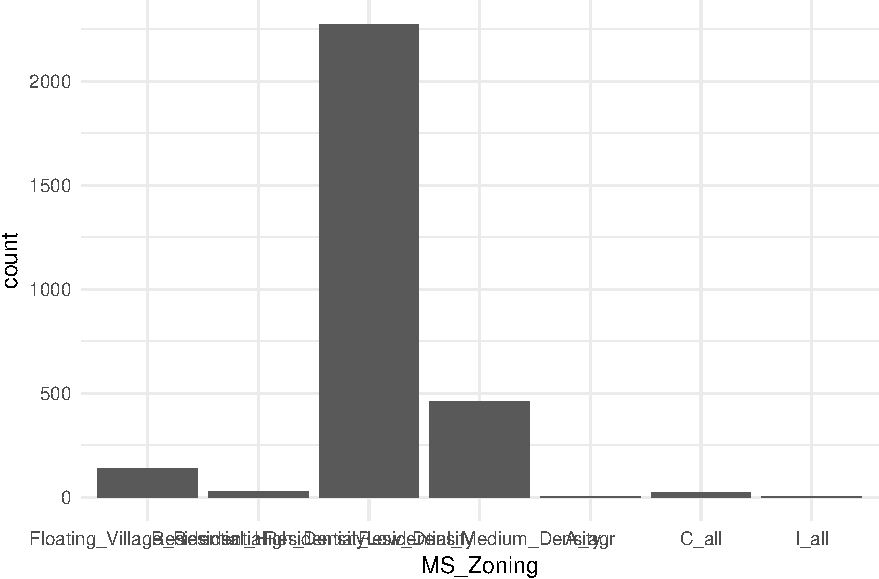
\includegraphics{Chapter_3_-_Visualization_files/figure-latex/bar1-1} \end{center}

Here, \texttt{MS\_Zoning} represents a nominal categorical variable
where there is no logical ordering of the labels; they simply represent
mutually exclusive levels within our variable. To get better clarity of
nominal variables we can make some refinements. Here I use
\texttt{dplyr::count} to count the observations in each level prior to
plotting. In the second plot I use \texttt{mutate} to compute the
percent that each level makes up of all observations. I then feed these
summarized data into \texttt{ggplot} where I can \texttt{reorder} the
\texttt{MS\_Zoning} variable from most frequent to least and then apply
\texttt{coord\_flip} to rotate the plot and make it easier to read the
level categories. Also, notice that now I feeding an x
(\texttt{MS\_Zoning}) and y (\texttt{n} in the left plot and
\texttt{pct} in the right plot) arguments so I apply \texttt{geom\_col}
rather than \texttt{geom\_bar}.

\begin{Shaded}
\begin{Highlighting}[]
\CommentTok{# total count}
\NormalTok{p1 <-}\StringTok{ }\NormalTok{ames }\OperatorTok\StringTok{ }
\StringTok{  }\KeywordTok{count}\NormalTok{(MS_Zoning) }\OperatorTok
\StringTok{  }\KeywordTok{ggplot}\NormalTok{(}\KeywordTok{aes}\NormalTok{(}\KeywordTok{reorder}\NormalTok{(MS_Zoning, n), n)) }\OperatorTok{+}
\StringTok{  }\KeywordTok{geom_col}\NormalTok{() }\OperatorTok{+}
\StringTok{  }\KeywordTok{coord_flip}\NormalTok{() }\OperatorTok{+}
\StringTok{  }\KeywordTok{ggtitle}\NormalTok{(}\StringTok{"Total count"}\NormalTok{)}

\CommentTok{# percent of whole}
\NormalTok{p2 <-}\StringTok{ }\NormalTok{ames }\OperatorTok\StringTok{ }
\StringTok{  }\KeywordTok{count}\NormalTok{(MS_Zoning) }\OperatorTok
\StringTok{  }\KeywordTok{mutate}\NormalTok{(}\DataTypeTok{pct =}\NormalTok{ n }\OperatorTok{/}\StringTok{ }\KeywordTok{sum}\NormalTok{(n)) }\OperatorTok
\StringTok{  }\KeywordTok{ggplot}\NormalTok{(}\KeywordTok{aes}\NormalTok{(}\KeywordTok{reorder}\NormalTok{(MS_Zoning, pct), pct)) }\OperatorTok{+}
\StringTok{  }\KeywordTok{geom_col}\NormalTok{() }\OperatorTok{+}
\StringTok{  }\KeywordTok{coord_flip}\NormalTok{() }\OperatorTok{+}
\StringTok{  }\KeywordTok{ggtitle}\NormalTok{(}\StringTok{"Percent of whole"}\NormalTok{)}

\NormalTok{gridExtra}\OperatorTok{::}\KeywordTok{grid.arrange}\NormalTok{(p1, p2, }\DataTypeTok{nrow =} \DecValTok{1}\NormalTok{)}
\end{Highlighting}
\end{Shaded}

\begin{center}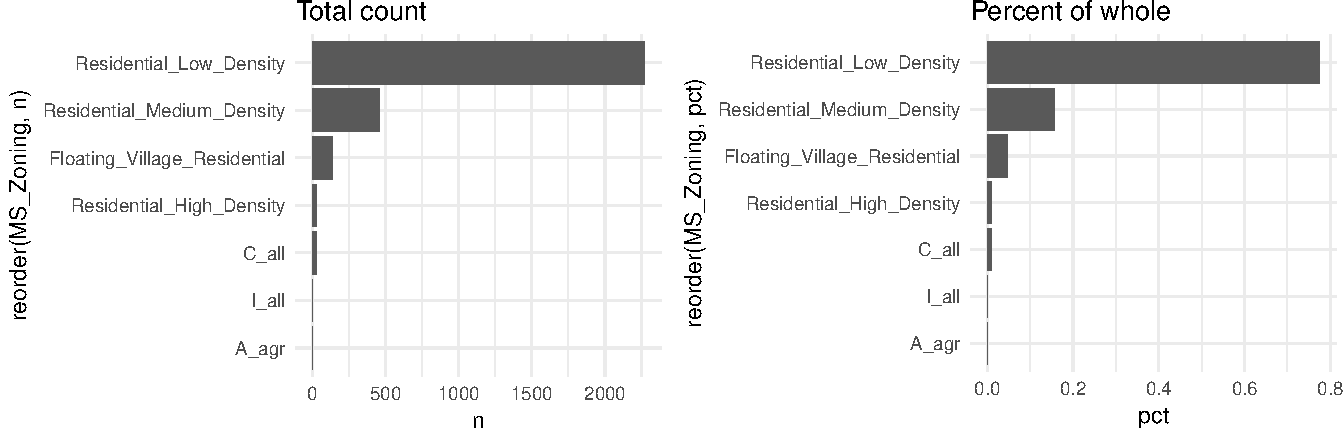
\includegraphics{Chapter_3_-_Visualization_files/figure-latex/bar2-1} \end{center}

Now we can see that properties zoned as residential low density make up
nearly 80\% of all observations . We also see that properties zoned as
aggricultural (\texttt{A\_agr}), industrial (\texttt{I\_all}),
commercial (\texttt{C\_all}), and residential high density make up a
very small amount of observations. In fact, below we see that these
imbalanced category levels each make up less than 1\% of all
observations.

\begin{Shaded}
\begin{Highlighting}[]
\NormalTok{ames }\OperatorTok\StringTok{ }
\StringTok{  }\KeywordTok{count}\NormalTok{(MS_Zoning) }\OperatorTok
\StringTok{  }\KeywordTok{mutate}\NormalTok{(}\DataTypeTok{pct =}\NormalTok{ n }\OperatorTok{/}\StringTok{ }\KeywordTok{sum}\NormalTok{(n)) }\OperatorTok
\StringTok{  }\KeywordTok{arrange}\NormalTok{(pct)}
\NormalTok{## # A tibble: 7 x 3}
\NormalTok{##   MS_Zoning                        n      pct}
\NormalTok{##   <fctr>                       <int>    <dbl>}
\NormalTok{## 1 A_agr                            2 0.000683}
\NormalTok{## 2 I_all                            2 0.000683}
\NormalTok{## 3 C_all                           25 0.00853 }
\NormalTok{## 4 Residential_High_Density        27 0.00922 }
\NormalTok{## 5 Floating_Village_Residential   139 0.0474  }
\NormalTok{## 6 Residential_Medium_Density     462 0.158   }
\NormalTok{## 7 Residential_Low_Density       2273 0.776}
\end{Highlighting}
\end{Shaded}

This imbalanced nature can cause problems in future analytic models so
it may make sense to combine these infrequent levels into an ``other''
category. An easy way to do that is to use \texttt{fct\_lump}.\footnote{A
  great resource to learn more about which you can learn more about
  managing factors is R for Data Science, Ch. 15.} Here we use
\texttt{n\ =\ 2} to retain the top 2 levels in our variable and condense
the remaining into an ``other'' category. You can see that this combined
category still represents less than 10\% of all observations.

\begin{Shaded}
\begin{Highlighting}[]
\NormalTok{ames }\OperatorTok\StringTok{ }
\StringTok{  }\KeywordTok{mutate}\NormalTok{(}\DataTypeTok{MS_Zoning =} \KeywordTok{fct_lump}\NormalTok{(MS_Zoning, }\DataTypeTok{n =} \DecValTok{2}\NormalTok{)) }\OperatorTok\StringTok{ }
\StringTok{  }\KeywordTok{count}\NormalTok{(MS_Zoning) }\OperatorTok
\StringTok{  }\KeywordTok{mutate}\NormalTok{(}\DataTypeTok{pct =}\NormalTok{ n }\OperatorTok{/}\StringTok{ }\KeywordTok{sum}\NormalTok{(n)) }\OperatorTok
\StringTok{  }\KeywordTok{ggplot}\NormalTok{(}\KeywordTok{aes}\NormalTok{(}\KeywordTok{reorder}\NormalTok{(MS_Zoning, pct), pct)) }\OperatorTok{+}
\StringTok{  }\KeywordTok{geom_col}\NormalTok{() }\OperatorTok{+}
\StringTok{  }\KeywordTok{coord_flip}\NormalTok{()}
\end{Highlighting}
\end{Shaded}

\begin{center}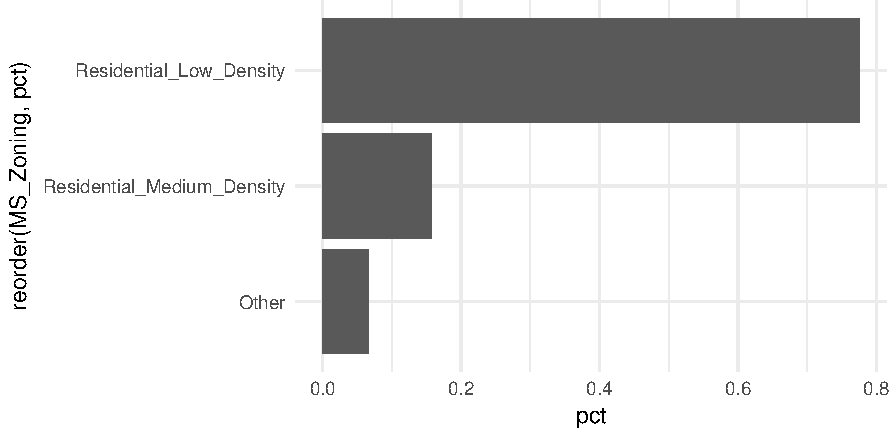
\includegraphics{Chapter_3_-_Visualization_files/figure-latex/bar3-1} \end{center}

Basic bar charts such as these are great when the number of category
levels is smaller. However, as the number of levels increase the thick
nature of the bar can be distracting. Cleveland dot plots and lollipop
charts are useful for assessing the frequency or proportion of many
levels while minizing the amount of ink on the graphic.

For example, if we assess the frequencies and proportions of home sales
by the 38 different neighborhoods a dotplot simplifies the chart.

\begin{Shaded}
\begin{Highlighting}[]
\NormalTok{ames }\OperatorTok\StringTok{  }
\StringTok{  }\KeywordTok{count}\NormalTok{(Neighborhood) }\OperatorTok
\StringTok{  }\KeywordTok{mutate}\NormalTok{(}\DataTypeTok{pct =}\NormalTok{ n }\OperatorTok{/}\StringTok{ }\KeywordTok{sum}\NormalTok{(n)) }\OperatorTok
\StringTok{  }\KeywordTok{ggplot}\NormalTok{(}\KeywordTok{aes}\NormalTok{(pct, }\KeywordTok{reorder}\NormalTok{(Neighborhood, pct))) }\OperatorTok{+}
\StringTok{  }\KeywordTok{geom_point}\NormalTok{()}
\end{Highlighting}
\end{Shaded}

\begin{center}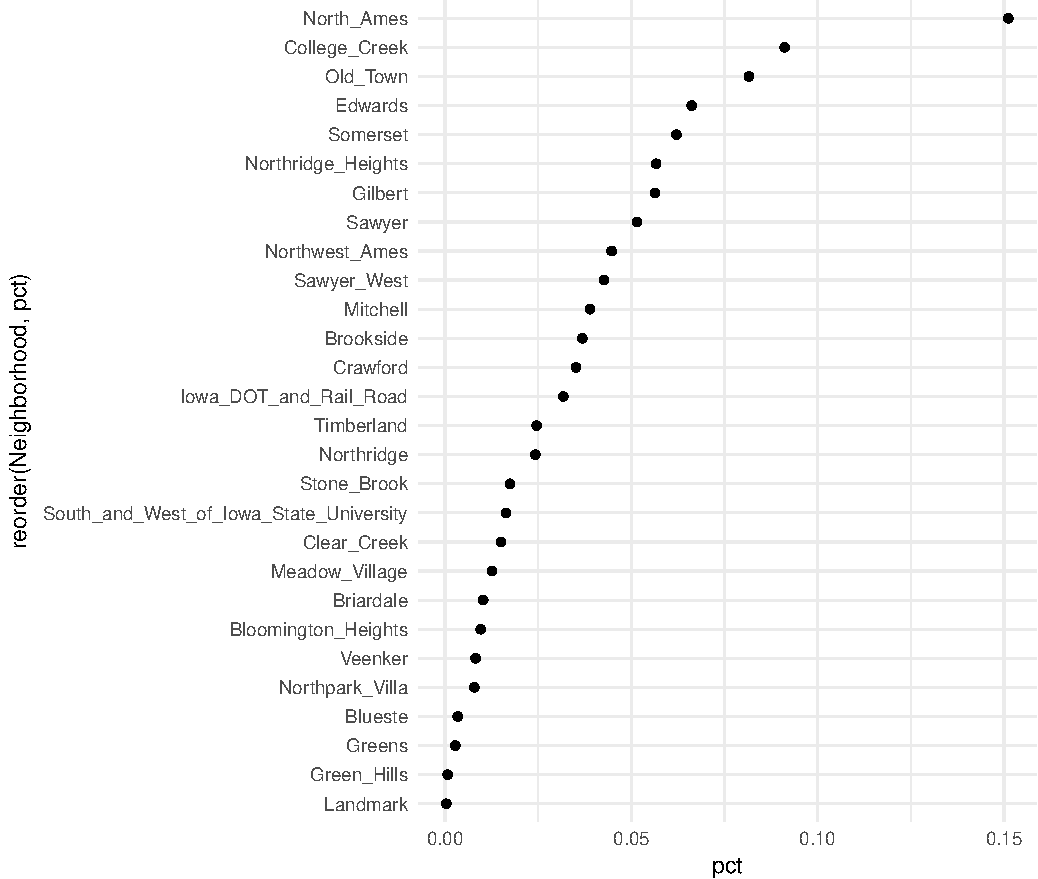
\includegraphics{Chapter_3_-_Visualization_files/figure-latex/dot-1} \end{center}

Similar to the Cleveland dot plot, a lollipop chart minimizes the visual
ink but uses a line to draw the readers attention to the specific x-axis
value achieved by each category. In the lollipop chart we use
\texttt{geom\_segment} to plot the lines and we explicitly state that we
want the lines to start at \texttt{x\ =\ 0} and extend to the
neighborhood value with \texttt{xend\ =\ pct}. We simply need to include
\texttt{y\ =\ neighborhood} and \texttt{yend\ =\ neighborhood} to tell R
the lines are horizontally attached to each neighborhood.

\begin{Shaded}
\begin{Highlighting}[]
\NormalTok{ames }\OperatorTok\StringTok{  }
\StringTok{  }\KeywordTok{count}\NormalTok{(Neighborhood) }\OperatorTok
\StringTok{  }\KeywordTok{mutate}\NormalTok{(}\DataTypeTok{pct =}\NormalTok{ n }\OperatorTok{/}\StringTok{ }\KeywordTok{sum}\NormalTok{(n)) }\OperatorTok
\StringTok{  }\KeywordTok{ggplot}\NormalTok{(}\KeywordTok{aes}\NormalTok{(pct, }\KeywordTok{reorder}\NormalTok{(Neighborhood, pct))) }\OperatorTok{+}
\StringTok{  }\KeywordTok{geom_point}\NormalTok{() }\OperatorTok{+}
\StringTok{  }\KeywordTok{geom_segment}\NormalTok{(}\KeywordTok{aes}\NormalTok{(}\DataTypeTok{x =} \DecValTok{0}\NormalTok{, }\DataTypeTok{xend =}\NormalTok{ pct, }\DataTypeTok{y =}\NormalTok{ Neighborhood, }\DataTypeTok{yend =}\NormalTok{ Neighborhood), }\DataTypeTok{size =}\NormalTok{ .}\DecValTok{15}\NormalTok{)}
\end{Highlighting}
\end{Shaded}

\begin{center}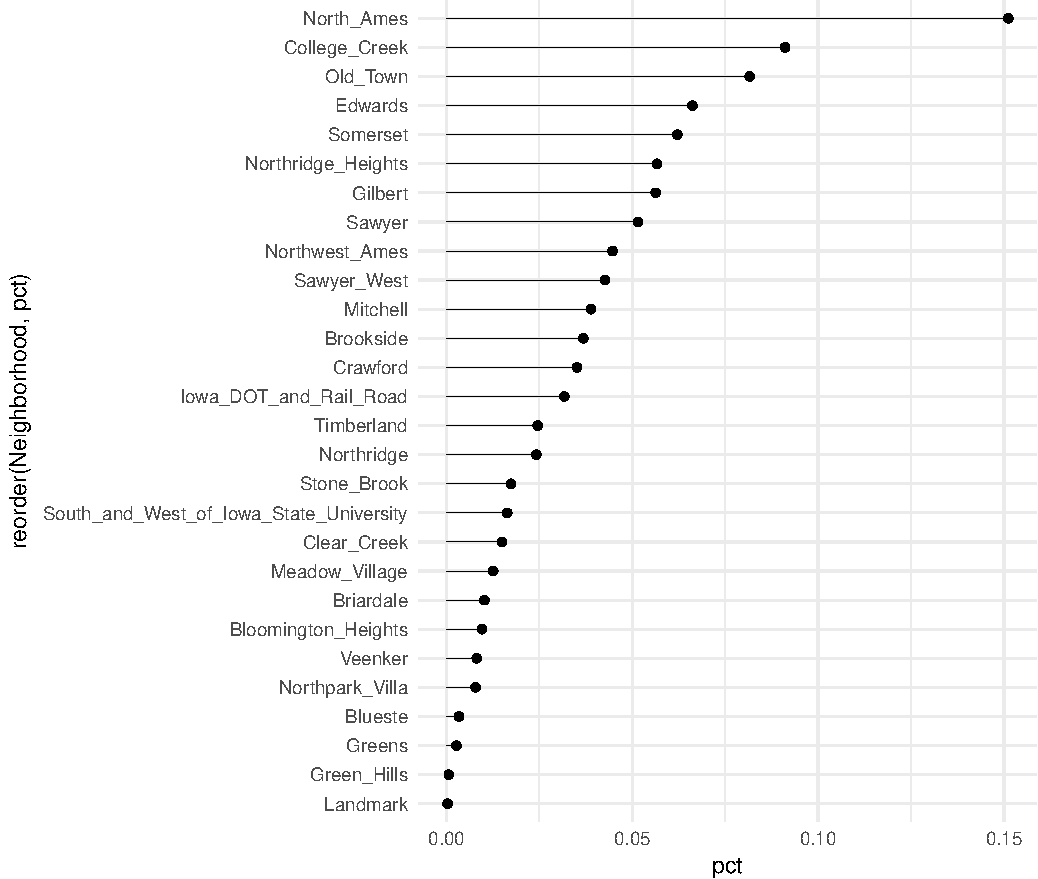
\includegraphics{Chapter_3_-_Visualization_files/figure-latex/dot1-1} \end{center}

Sometimes we have categorical data that have natural, ordered
categories. These types of categorical variables can be ordinal or
interval. An ordinal variable is one in which the order of the values
can be important but the differences between each one is not really
known. For example, our \texttt{ames} data categorizes the quality of
kitchens into five buckets and these buckets have a natural order that
is not captured with a regular bar chart.

\begin{Shaded}
\begin{Highlighting}[]
\KeywordTok{ggplot}\NormalTok{(ames, }\KeywordTok{aes}\NormalTok{(Kitchen_Qual)) }\OperatorTok{+}\StringTok{ }
\StringTok{  }\KeywordTok{geom_bar}\NormalTok{()}
\end{Highlighting}
\end{Shaded}

\begin{center}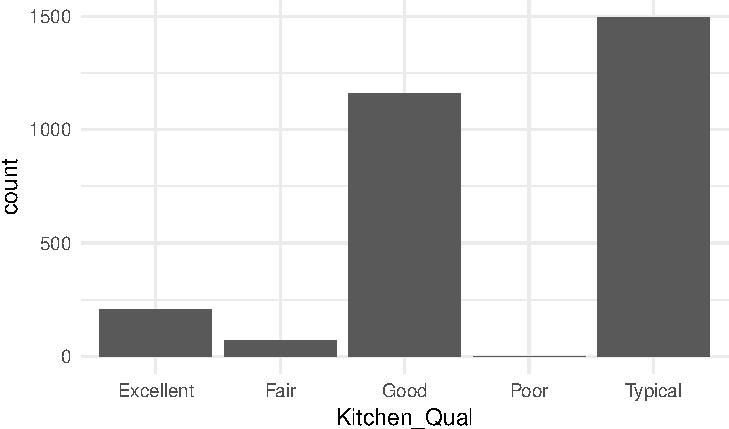
\includegraphics{Chapter_3_-_Visualization_files/figure-latex/ord1-1} \end{center}

Here, rather than order by frequency it may be important to order the
bars by the natural order of the quality lables: Poor, Fair, Typical,
Good, Excellent. This can provide better insight into where most
observations fall within this spectrum of quality. To do this we reorder
the factor levels with \texttt{fct\_relevel} and now its easier to see
that most homes have average to slightly above average quality kitchens.

\begin{Shaded}
\begin{Highlighting}[]
\NormalTok{ames }\OperatorTok
\StringTok{  }\KeywordTok{mutate}\NormalTok{(}\DataTypeTok{Kitchen_Qual =} \KeywordTok{fct_relevel}\NormalTok{(Kitchen_Qual, }\StringTok{"Poor"}\NormalTok{, }\StringTok{"Fair"}\NormalTok{, }\StringTok{"Typical"}\NormalTok{, }\StringTok{"Good"}\NormalTok{)) }\OperatorTok
\StringTok{  }\KeywordTok{ggplot}\NormalTok{(}\KeywordTok{aes}\NormalTok{(Kitchen_Qual)) }\OperatorTok{+}\StringTok{ }
\StringTok{  }\KeywordTok{geom_bar}\NormalTok{()}
\end{Highlighting}
\end{Shaded}

\begin{center}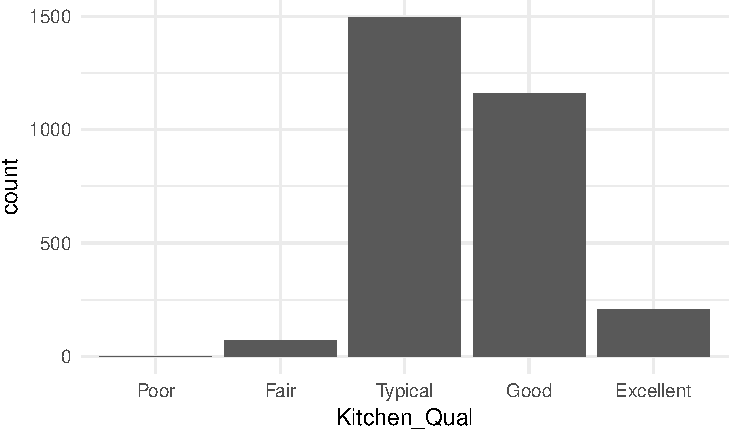
\includegraphics{Chapter_3_-_Visualization_files/figure-latex/ord2-1} \end{center}

We may also have a categorical variable that has set intervals and may
even be identified by integer values. For example, our data identifies
the month each home was sold but uses integer values to represent the
months. In this case we do not need to reorder our factor levels but we
should ensure we visualize these as discrete factor levels (note how I
apply \texttt{factor(Mo\_Sold)} within ggplot) so that the home sale
counts are appropriately bucketed into each month.

\begin{Shaded}
\begin{Highlighting}[]
\NormalTok{p1 <-}\StringTok{ }\KeywordTok{ggplot}\NormalTok{(ames, }\KeywordTok{aes}\NormalTok{(Mo_Sold)) }\OperatorTok{+}\StringTok{ }
\StringTok{  }\KeywordTok{geom_bar}\NormalTok{()}

\NormalTok{p2 <-}\StringTok{ }\KeywordTok{ggplot}\NormalTok{(ames, }\KeywordTok{aes}\NormalTok{(}\KeywordTok{factor}\NormalTok{(Mo_Sold))) }\OperatorTok{+}\StringTok{ }
\StringTok{  }\KeywordTok{geom_bar}\NormalTok{()}

\NormalTok{gridExtra}\OperatorTok{::}\KeywordTok{grid.arrange}\NormalTok{(p1, p2, }\DataTypeTok{nrow =} \DecValTok{2}\NormalTok{)}
\end{Highlighting}
\end{Shaded}

\begin{center}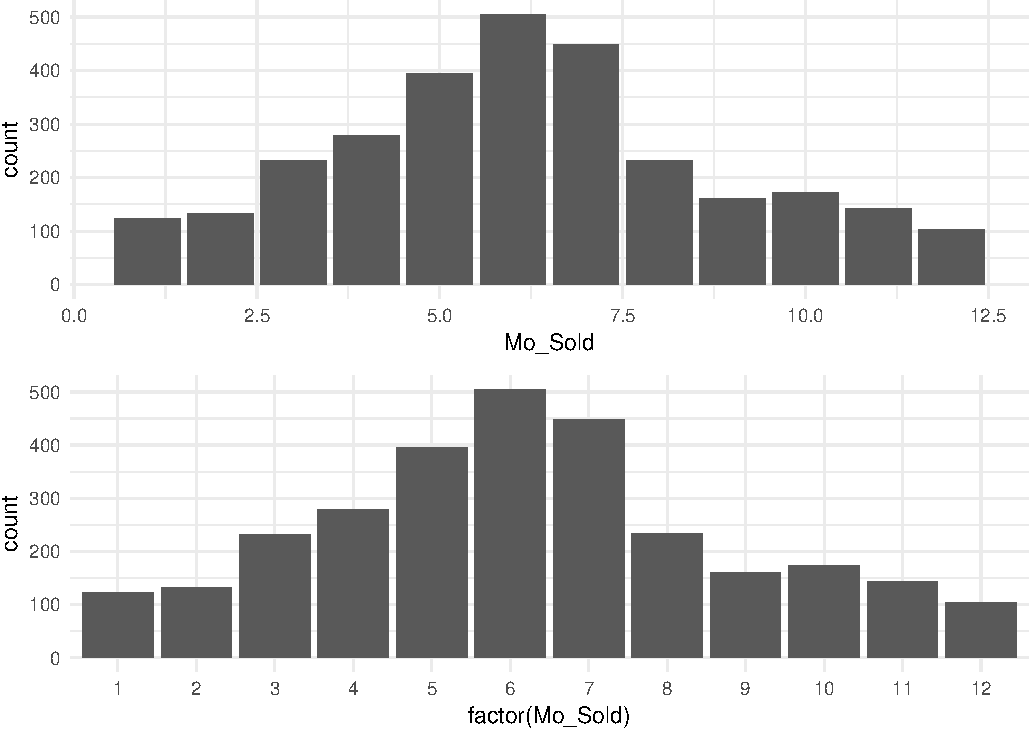
\includegraphics{Chapter_3_-_Visualization_files/figure-latex/int1-1} \end{center}

Bar charts can also illustrate how our missing values are disbursed
across categorical variables. Using the \texttt{MASS::survey} data
(since our \texttt{ames} data does not have any missing data) we can
make small multiples (more on this in the next section) using
\texttt{facet\_wrap} to visualize the \texttt{NA}s.

\begin{Shaded}
\begin{Highlighting}[]
\NormalTok{MASS}\OperatorTok{::}\NormalTok{survey }\OperatorTok
\StringTok{  }\KeywordTok{select}\NormalTok{(Sex, Exer, Smoke, Fold, Clap, M.I) }\OperatorTok
\StringTok{  }\KeywordTok{gather}\NormalTok{(var, value, Sex}\OperatorTok{:}\NormalTok{M.I) }\OperatorTok
\StringTok{  }\KeywordTok{ggplot}\NormalTok{(}\KeywordTok{aes}\NormalTok{(value)) }\OperatorTok{+}
\StringTok{  }\KeywordTok{geom_bar}\NormalTok{() }\OperatorTok{+}
\StringTok{  }\KeywordTok{facet_wrap}\NormalTok{(}\OperatorTok{~}\StringTok{ }\NormalTok{var, }\DataTypeTok{scales =} \StringTok{"free"}\NormalTok{)}
\end{Highlighting}
\end{Shaded}

\begin{center}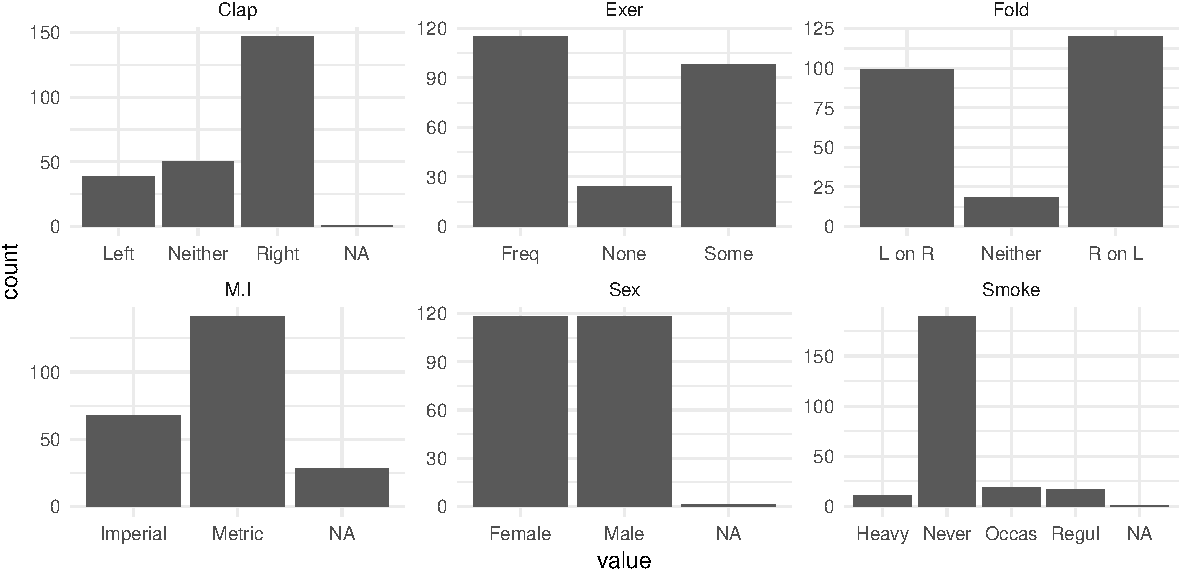
\includegraphics{Chapter_3_-_Visualization_files/figure-latex/missing1-1} \end{center}

Or in some cases observations are not labeled correctly. If we look at
the \texttt{Embarked} variable in the \texttt{titanic} package we see
that the levels are labeled as C, Q, and S; however, there are two cases
that have no label (these values are coded as \texttt{""} in the actual
data set). These are missing values that are just not coded as
\texttt{NA}s. For modeling purposes we would likely recode these as
either \texttt{NA}s or impute them as one of the other three levels (C,
Q, or S).

\begin{Shaded}
\begin{Highlighting}[]
\KeywordTok{ggplot}\NormalTok{(titanic}\OperatorTok{::}\NormalTok{titanic_train, }\KeywordTok{aes}\NormalTok{(Embarked)) }\OperatorTok{+}
\StringTok{  }\KeywordTok{geom_bar}\NormalTok{()}
\end{Highlighting}
\end{Shaded}

\begin{center}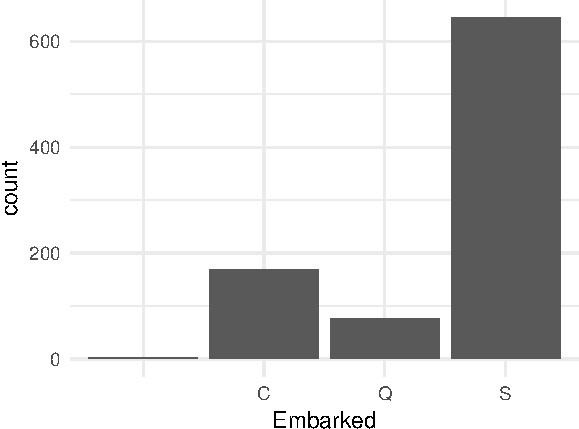
\includegraphics{Chapter_3_-_Visualization_files/figure-latex/mislabeled-1} \end{center}

Bar charts and their cousins are a simple form of visual display, yet
they can provide much information about our categorical variables.
Whether viewing nominal, ordinal, or interval data we can make minor
adjustments in our bar charts to highlight the important features of our
variables.

\section{Relationships and
Associations}\label{relationships-and-associations}

Having a solid understanding of univariate distributions is important;
however, most analyses want to take the next step to understand
associations and relationships between variables. Features we are
generally interested in include:

\begin{itemize}
\tightlist
\item
  Associations
\item
  Outliers
\item
  Clusters
\item
  Gaps
\item
  Barriers
\item
  Change points
\end{itemize}

One of the most popular plots to assess association is the scatter plot.
The scatter plot helps us to see multiple features between two
continuous variables. Here we look at the relationship between
\texttt{Sale\_Price} and total above ground square footage
(\texttt{Gr\_Liv\_Area}). A few features that pop out from this plot
includes:

\begin{itemize}
\tightlist
\item
  Associations: There is a positive relationship between these two
  variables. As total above ground square footage increases the sale
  price also increases.
\item
  Outliers: Several outliers appear in multiple directions. Two outliers
  appear at the top of the chart suggesting these are larger than normal
  homes that sold for very high prices. We also see three outliers at
  the far right of the chart suggesting these homes have very large
  square footage but sold for average sale prices.
\item
  Clusters: Give the large number of points there is a lot of
  overplotting, which is why I incorporated \texttt{alpha\ =\ .3} to
  increase transparency. This allows us to see the clustering of data
  points in the center of the variable relationship.
\item
  Barriers: The outer limits of our point clustering shows us that there
  are limitations on the sale price for given ranges of square footage.
  For example, homes with less than 1,000 square feet above ground
  appear to have a price ceiling of \$200,000 or less.
\end{itemize}

\begin{Shaded}
\begin{Highlighting}[]
\KeywordTok{ggplot}\NormalTok{(ames, }\KeywordTok{aes}\NormalTok{(}\DataTypeTok{x =}\NormalTok{ Gr_Liv_Area, }\DataTypeTok{y =}\NormalTok{ Sale_Price)) }\OperatorTok{+}
\StringTok{  }\KeywordTok{geom_point}\NormalTok{(}\DataTypeTok{alpha =}\NormalTok{ .}\DecValTok{3}\NormalTok{)}
\end{Highlighting}
\end{Shaded}

\begin{center}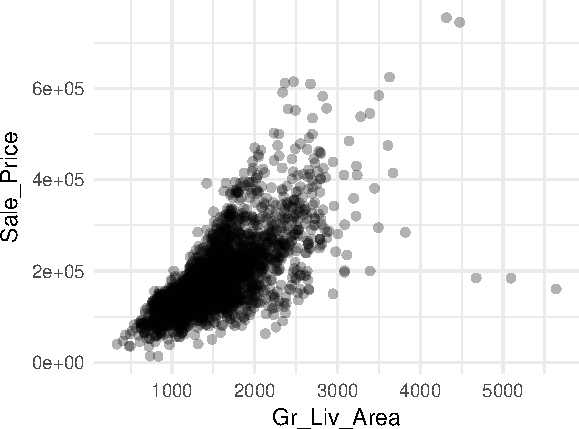
\includegraphics{Chapter_3_-_Visualization_files/figure-latex/scatter1-1} \end{center}

This relationship appears to be fairly linear but it is unclear. We can
add trend lines to assess the linearity. In the below plot we add a
linear line with \texttt{geom\_smooth(method\ =\ "lm")} (note the
\texttt{method\ =\ "lm"} means to add a linear model line) and then we
add a non-linear line (the second \texttt{geom\_smooth} without a
specified \texttt{method} adds uses a generalized additive model). This
allows us to assess how non-linear a relationship may be. Our new plot
shows that for homes with less than 2,250 square feet the relationship
is fairly linear; however, beyond 2,250 square feet we see strong
deviations from linearity.

Also, note the funneling in the left scatter plot. This is called
heteroskedasticity (non-constant variance) and this can cause concerns
with certain future modeling approaches (i.e.~forms of linear
regression). We can assess if transforming our variables can alleviate
this concern by adding \texttt{scale\_?\_log10}. The right plot shows
that transforming our variables makes our variability across the plot
more constant. We see that for the majority of the plot the relationship
is now linear with the exception of the two ends where we see the
non-linear line being pulled down. This suggests that there are some
influential observations with low and high square footage that are
pulling the expected sale price down.

\begin{Shaded}
\begin{Highlighting}[]
\NormalTok{p1 <-}\StringTok{ }\KeywordTok{ggplot}\NormalTok{(ames, }\KeywordTok{aes}\NormalTok{(}\DataTypeTok{x =}\NormalTok{ Gr_Liv_Area, }\DataTypeTok{y =}\NormalTok{ Sale_Price)) }\OperatorTok{+}
\StringTok{  }\KeywordTok{geom_point}\NormalTok{(}\DataTypeTok{alpha =}\NormalTok{ .}\DecValTok{3}\NormalTok{) }\OperatorTok{+}
\StringTok{  }\KeywordTok{geom_smooth}\NormalTok{(}\DataTypeTok{method =} \StringTok{"lm"}\NormalTok{, }\DataTypeTok{se =} \OtherTok{FALSE}\NormalTok{, }\DataTypeTok{color =} \StringTok{"red"}\NormalTok{, }\DataTypeTok{lty =} \StringTok{"dashed"}\NormalTok{) }\OperatorTok{+}
\StringTok{  }\KeywordTok{geom_smooth}\NormalTok{(}\DataTypeTok{se =} \OtherTok{FALSE}\NormalTok{, }\DataTypeTok{lty =} \StringTok{"dashed"}\NormalTok{) }\OperatorTok{+}
\StringTok{  }\KeywordTok{ggtitle}\NormalTok{(}\StringTok{"Non-transformed variables"}\NormalTok{)}

\NormalTok{p2 <-}\StringTok{ }\KeywordTok{ggplot}\NormalTok{(ames, }\KeywordTok{aes}\NormalTok{(}\DataTypeTok{x =}\NormalTok{ Gr_Liv_Area, }\DataTypeTok{y =}\NormalTok{ Sale_Price)) }\OperatorTok{+}
\StringTok{  }\KeywordTok{geom_point}\NormalTok{(}\DataTypeTok{alpha =}\NormalTok{ .}\DecValTok{3}\NormalTok{) }\OperatorTok{+}
\StringTok{  }\KeywordTok{geom_smooth}\NormalTok{(}\DataTypeTok{method =} \StringTok{"lm"}\NormalTok{, }\DataTypeTok{se =} \OtherTok{FALSE}\NormalTok{, }\DataTypeTok{color =} \StringTok{"red"}\NormalTok{, }\DataTypeTok{lty =} \StringTok{"dashed"}\NormalTok{) }\OperatorTok{+}
\StringTok{  }\KeywordTok{geom_smooth}\NormalTok{(}\DataTypeTok{se =} \OtherTok{FALSE}\NormalTok{, }\DataTypeTok{lty =} \StringTok{"dashed"}\NormalTok{) }\OperatorTok{+}
\StringTok{  }\KeywordTok{scale_x_log10}\NormalTok{() }\OperatorTok{+}
\StringTok{  }\KeywordTok{scale_y_log10}\NormalTok{() }\OperatorTok{+}
\StringTok{  }\KeywordTok{ggtitle}\NormalTok{(}\StringTok{"log-transformed variables"}\NormalTok{)}

\NormalTok{gridExtra}\OperatorTok{::}\KeywordTok{grid.arrange}\NormalTok{(p1, p2, }\DataTypeTok{nrow =} \DecValTok{1}\NormalTok{)}
\end{Highlighting}
\end{Shaded}

\begin{center}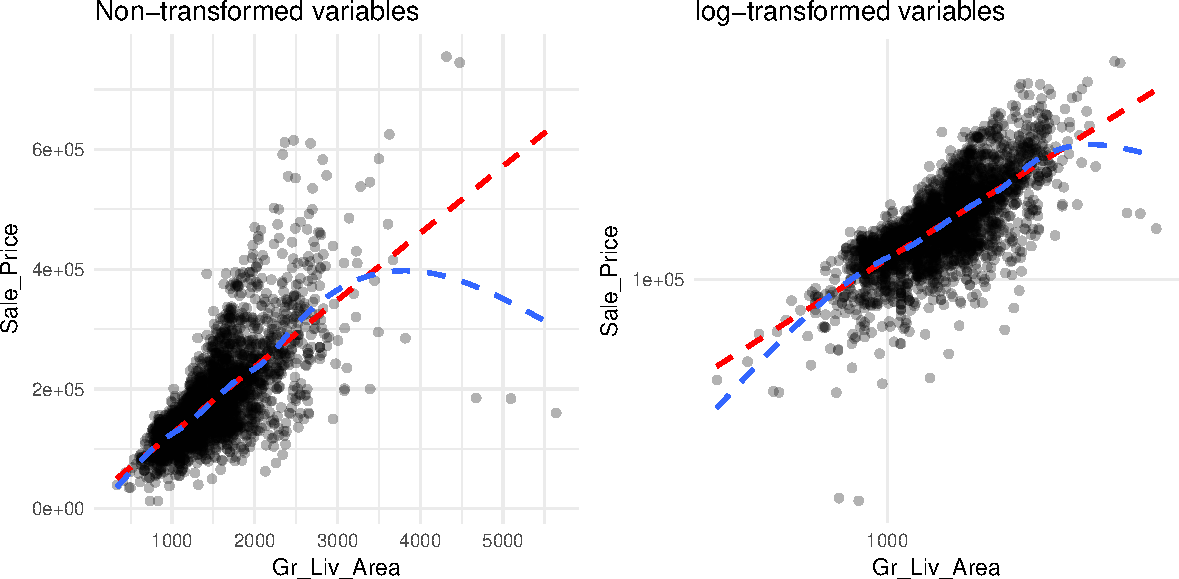
\includegraphics{Chapter_3_-_Visualization_files/figure-latex/dbl_scatter-1} \end{center}

Scatter plots can also signal distinct clustering or gaps. For example,
if we plot \texttt{Sale\_Price} versus \texttt{Garage\_Area} (left) we
see a couple areas of concentrated points. By incorporating a density
plot (middle) we can draw attention to the centers of these clusters
which appears to be located at homes with zero garage square footage and
homes with just over 250 square feet and just under 500 square feet of
garage area. We can also change our plot to a hexbin plot, that replaces
bunches of points with a larger hexagonal symbol. This provides us with
a heatmap-like plot to signal highly concentrated regions. It also does
a better job identifying gaps in our data where no observations exist.

\begin{Shaded}
\begin{Highlighting}[]
\NormalTok{p1 <-}\StringTok{ }\KeywordTok{ggplot}\NormalTok{(ames, }\KeywordTok{aes}\NormalTok{(}\DataTypeTok{x =}\NormalTok{ Garage_Area, }\DataTypeTok{y =}\NormalTok{ Sale_Price)) }\OperatorTok{+}\StringTok{ }
\StringTok{  }\KeywordTok{geom_point}\NormalTok{(}\DataTypeTok{alpha =}\NormalTok{ .}\DecValTok{2}\NormalTok{)}

\NormalTok{p2 <-}\StringTok{ }\KeywordTok{ggplot}\NormalTok{(ames, }\KeywordTok{aes}\NormalTok{(}\DataTypeTok{x =}\NormalTok{ Garage_Area, }\DataTypeTok{y =}\NormalTok{ Sale_Price)) }\OperatorTok{+}\StringTok{ }
\StringTok{  }\KeywordTok{geom_point}\NormalTok{(}\DataTypeTok{alpha =}\NormalTok{ .}\DecValTok{2}\NormalTok{) }\OperatorTok{+}\StringTok{ }
\StringTok{  }\KeywordTok{geom_density2d}\NormalTok{()}

\NormalTok{p3 <-}\StringTok{ }\KeywordTok{ggplot}\NormalTok{(ames, }\KeywordTok{aes}\NormalTok{(}\DataTypeTok{x =}\NormalTok{ Garage_Area, }\DataTypeTok{y =}\NormalTok{ Sale_Price)) }\OperatorTok{+}\StringTok{ }
\StringTok{  }\KeywordTok{geom_hex}\NormalTok{(}\DataTypeTok{bins =} \DecValTok{50}\NormalTok{, }\DataTypeTok{show.legend =} \OtherTok{FALSE}\NormalTok{)}

\NormalTok{gridExtra}\OperatorTok{::}\KeywordTok{grid.arrange}\NormalTok{(p1, p2, p3, }\DataTypeTok{nrow =} \DecValTok{1}\NormalTok{)}
\end{Highlighting}
\end{Shaded}

\begin{center}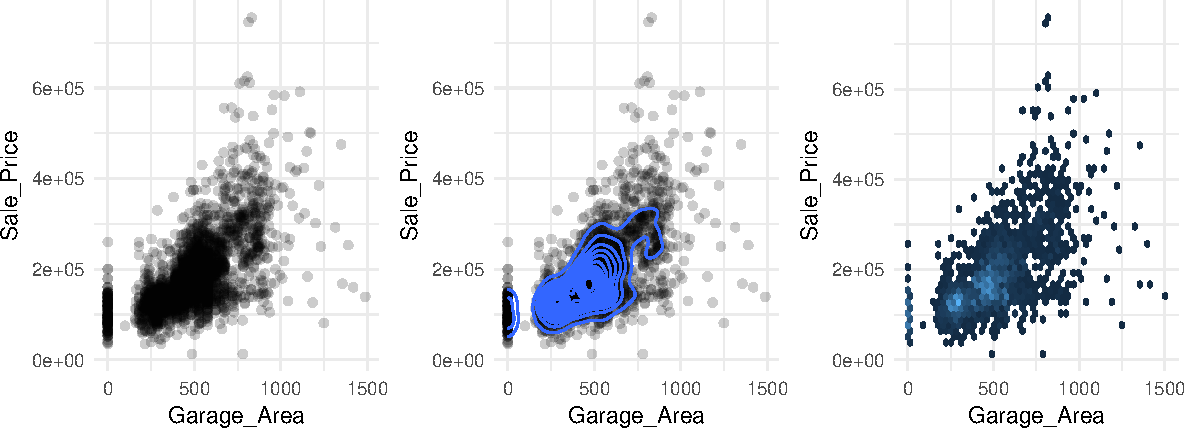
\includegraphics{Chapter_3_-_Visualization_files/figure-latex/density_plot-1} \end{center}

When using a scatter plot to assess a continuous variable against a
categorical variable a stip plot will form. Here we assess the
\texttt{Sale\_Price} to the number of above ground bedrooms
(\texttt{Bedroom\_AbvGr}). Due to the size of this data set, the top
left strip plot has a lot of overlaid data points. We can use
\texttt{geom\_jitter} to add a little variation to our plot (top right),
which allows us to see where heavier concentrations of points exist.
Alternatively, we can use boxplots and violin plots to compare the
distributions of \texttt{Sale\_Price} to \texttt{Bedroom\_AbvGr}. Each
plot provides different insights to the different features
(i.e.~outliers, clustering, median values).

\begin{Shaded}
\begin{Highlighting}[]
\NormalTok{p1 <-}\StringTok{ }\KeywordTok{ggplot}\NormalTok{(ames, }\KeywordTok{aes}\NormalTok{(}\DataTypeTok{x =} \KeywordTok{factor}\NormalTok{(Bedroom_AbvGr), }\DataTypeTok{y =}\NormalTok{ Sale_Price)) }\OperatorTok{+}
\StringTok{  }\KeywordTok{geom_point}\NormalTok{(}\DataTypeTok{alpha =}\NormalTok{ .}\DecValTok{3}\NormalTok{)}

\NormalTok{p2 <-}\StringTok{ }\KeywordTok{ggplot}\NormalTok{(ames, }\KeywordTok{aes}\NormalTok{(}\DataTypeTok{x =} \KeywordTok{factor}\NormalTok{(Bedroom_AbvGr), }\DataTypeTok{y =}\NormalTok{ Sale_Price)) }\OperatorTok{+}
\StringTok{  }\KeywordTok{geom_jitter}\NormalTok{(}\DataTypeTok{alpha =}\NormalTok{ .}\DecValTok{5}\NormalTok{, }\DataTypeTok{width =}\NormalTok{ .}\DecValTok{2}\NormalTok{)}

\NormalTok{p3 <-}\StringTok{ }\KeywordTok{ggplot}\NormalTok{(ames, }\KeywordTok{aes}\NormalTok{(}\DataTypeTok{x =} \KeywordTok{factor}\NormalTok{(Bedroom_AbvGr), }\DataTypeTok{y =}\NormalTok{ Sale_Price)) }\OperatorTok{+}
\StringTok{  }\KeywordTok{geom_boxplot}\NormalTok{()}

\NormalTok{p4 <-}\StringTok{ }\KeywordTok{ggplot}\NormalTok{(ames, }\KeywordTok{aes}\NormalTok{(}\DataTypeTok{x =} \KeywordTok{factor}\NormalTok{(Bedroom_AbvGr), }\DataTypeTok{y =}\NormalTok{ Sale_Price)) }\OperatorTok{+}
\StringTok{  }\KeywordTok{geom_violin}\NormalTok{()}

\NormalTok{gridExtra}\OperatorTok{::}\KeywordTok{grid.arrange}\NormalTok{(p1, p2, p3, p4, }\DataTypeTok{nrow =} \DecValTok{2}\NormalTok{)}
\end{Highlighting}
\end{Shaded}

\begin{center}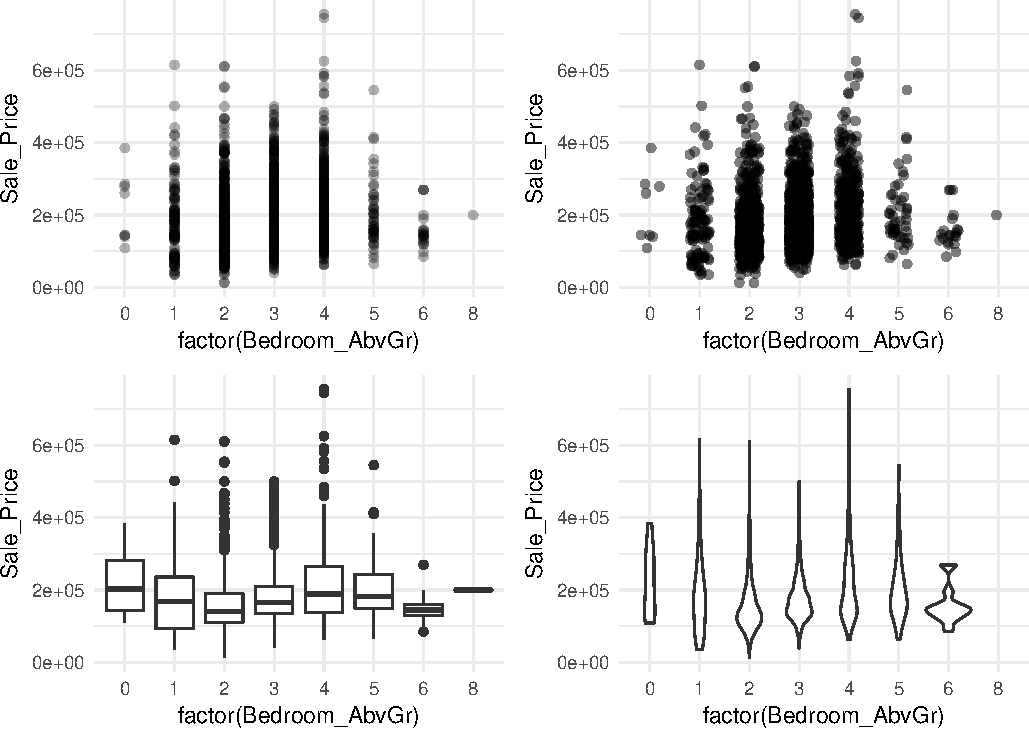
\includegraphics{Chapter_3_-_Visualization_files/figure-latex/int_scatter-1} \end{center}

An alternative approach to view the distribution of a continuous
variable across multiple categories includes overlaying distribution
plots. For example, we could assess the \texttt{Sale\_Price} of homes
across the overall quality of homes. We can do this with a frequency
polygon (left), which display the outline of a histogram. However, since
some quality levels have very low counts it is tough to see the
distribution of costs within each category. A better approach is to
overlay density plots which allows us to see how each quality level's
distribution differs from one another.

\begin{Shaded}
\begin{Highlighting}[]
\NormalTok{p1 <-}\StringTok{ }\KeywordTok{ggplot}\NormalTok{(ames, }\KeywordTok{aes}\NormalTok{(}\DataTypeTok{x =}\NormalTok{ Sale_Price, }\DataTypeTok{color =}\NormalTok{ Overall_Qual)) }\OperatorTok{+}
\StringTok{  }\KeywordTok{geom_freqpoly}\NormalTok{() }\OperatorTok{+}
\StringTok{  }\KeywordTok{scale_x_log10}\NormalTok{(}\DataTypeTok{breaks =} \KeywordTok{c}\NormalTok{(}\DecValTok{50}\NormalTok{, }\DecValTok{150}\NormalTok{, }\DecValTok{400}\NormalTok{, }\DecValTok{750}\NormalTok{) }\OperatorTok{*}\StringTok{ }\DecValTok{1000}\NormalTok{, }\DataTypeTok{labels =}\NormalTok{ scales}\OperatorTok{::}\NormalTok{dollar)}
  
\NormalTok{p2 <-}\StringTok{ }\KeywordTok{ggplot}\NormalTok{(ames, }\KeywordTok{aes}\NormalTok{(}\DataTypeTok{x =}\NormalTok{ Sale_Price, }\DataTypeTok{color =}\NormalTok{ Overall_Qual, }\DataTypeTok{fill =}\NormalTok{ Overall_Qual)) }\OperatorTok{+}
\StringTok{  }\KeywordTok{geom_density}\NormalTok{(}\DataTypeTok{alpha =}\NormalTok{ .}\DecValTok{15}\NormalTok{) }\OperatorTok{+}
\StringTok{  }\KeywordTok{scale_x_log10}\NormalTok{(}\DataTypeTok{breaks =} \KeywordTok{c}\NormalTok{(}\DecValTok{50}\NormalTok{, }\DecValTok{150}\NormalTok{, }\DecValTok{400}\NormalTok{, }\DecValTok{750}\NormalTok{) }\OperatorTok{*}\StringTok{ }\DecValTok{1000}\NormalTok{, }\DataTypeTok{labels =}\NormalTok{ scales}\OperatorTok{::}\NormalTok{dollar)}

\NormalTok{gridExtra}\OperatorTok{::}\KeywordTok{grid.arrange}\NormalTok{(p1, p2, }\DataTypeTok{nrow =} \DecValTok{2}\NormalTok{)}
\end{Highlighting}
\end{Shaded}

\begin{center}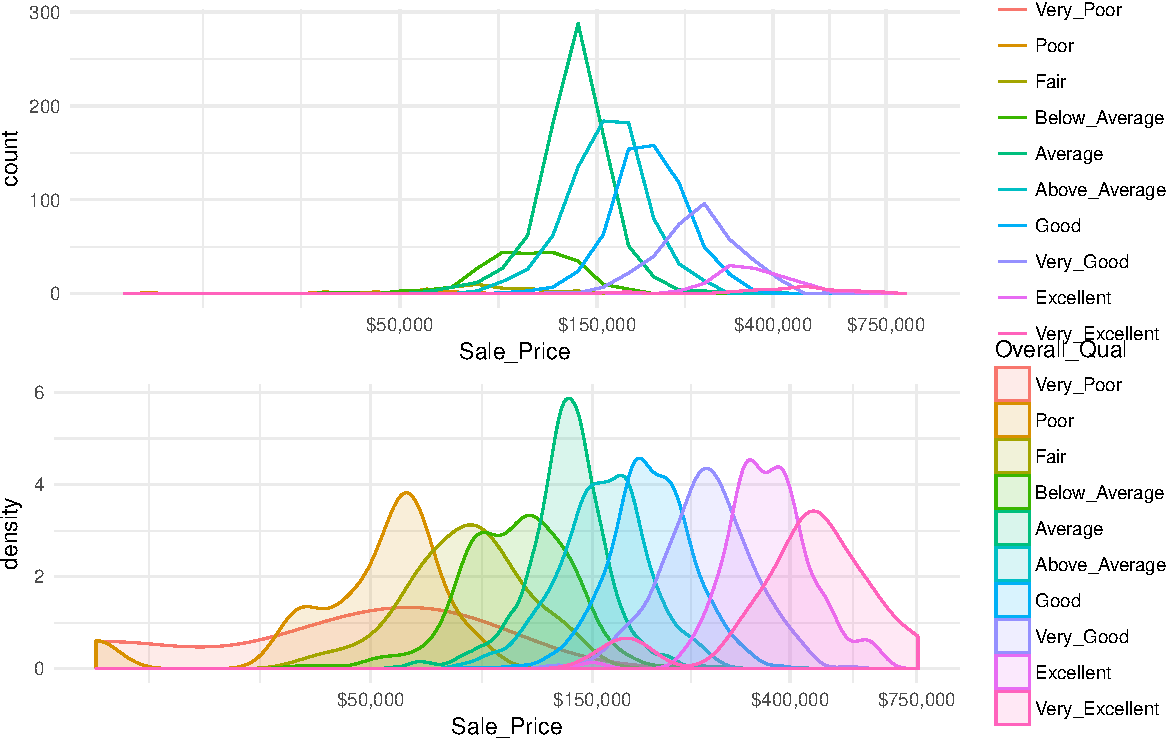
\includegraphics{Chapter_3_-_Visualization_files/figure-latex/unnamed-chunk-3-1} \end{center}

When there are many levels in a categorical variable, overlaid plots
become difficult to decipher. Rather than overlay plots, we can also use
small multiples to compare the distribution of a continuous variable.
Joyplots provide a form of small multiples by partially overlapping
distribution plots. They can be quite useful for visualizing changes in
continuous distributions over discrete variable levels. In this example
I use the \texttt{ggjoy} package which provides an add-on
\texttt{geom\_joy} for ggplot. Now we get a much clearer picture how the
sales price differs for each quality level.

\begin{Shaded}
\begin{Highlighting}[]
\KeywordTok{ggplot}\NormalTok{(ames, }\KeywordTok{aes}\NormalTok{(}\DataTypeTok{x =}\NormalTok{ Sale_Price, }\DataTypeTok{y =}\NormalTok{ Overall_Qual)) }\OperatorTok{+}\StringTok{ }
\StringTok{  }\NormalTok{ggjoy}\OperatorTok{::}\KeywordTok{geom_joy}\NormalTok{() }\OperatorTok{+}
\StringTok{  }\KeywordTok{scale_x_continuous}\NormalTok{(}\DataTypeTok{labels =}\NormalTok{ scales}\OperatorTok{::}\NormalTok{dollar)}
\end{Highlighting}
\end{Shaded}

\begin{center}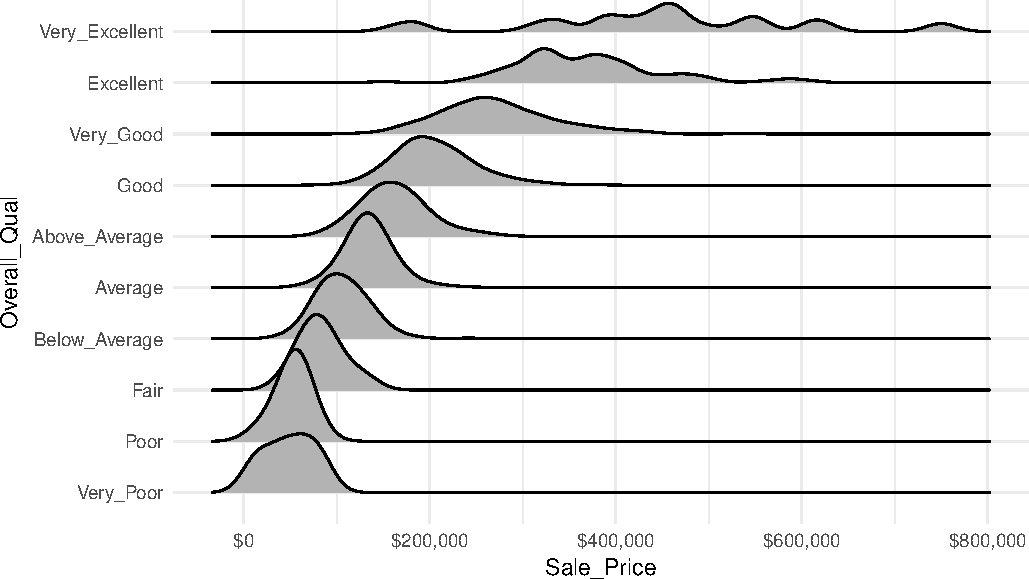
\includegraphics{Chapter_3_-_Visualization_files/figure-latex/joyplot-1} \end{center}

It is important to understand how a categorical response is associated
with multiple variables. We can use faceting (\texttt{facet\_wrap} and
\texttt{facet\_grid}) to produce small multiples of bar charts across
the levels of 1 or more categorical variable. For example, here we
assess the quality of kitchens for homes that sold above and below the
mean sales price. Not surprisingly we see homes above average sales
price have higher quality kitchens.

\begin{Shaded}
\begin{Highlighting}[]
\NormalTok{ames }\OperatorTok
\StringTok{  }\KeywordTok{mutate}\NormalTok{(}
    \DataTypeTok{Above_Avg =} \KeywordTok{ifelse}\NormalTok{(Sale_Price }\OperatorTok{>}\StringTok{ }\KeywordTok{mean}\NormalTok{(Sale_Price), }\StringTok{"Above"}\NormalTok{, }\StringTok{"Below"}\NormalTok{),}
    \DataTypeTok{Kitchen_Qual =} \KeywordTok{fct_relevel}\NormalTok{(Kitchen_Qual, }\StringTok{"Poor"}\NormalTok{, }\StringTok{"Fair"}\NormalTok{, }\StringTok{"Typical"}\NormalTok{, }\StringTok{"Good"}\NormalTok{)}
\NormalTok{    ) }\OperatorTok
\StringTok{  }\KeywordTok{ggplot}\NormalTok{(}\KeywordTok{aes}\NormalTok{(Kitchen_Qual)) }\OperatorTok{+}\StringTok{ }
\StringTok{  }\KeywordTok{geom_bar}\NormalTok{() }\OperatorTok{+}
\StringTok{  }\KeywordTok{facet_wrap}\NormalTok{(}\OperatorTok{~}\StringTok{ }\NormalTok{Above_Avg) }\OperatorTok{+}
\StringTok{  }\KeywordTok{theme_bw}\NormalTok{()}
\end{Highlighting}
\end{Shaded}

\begin{center}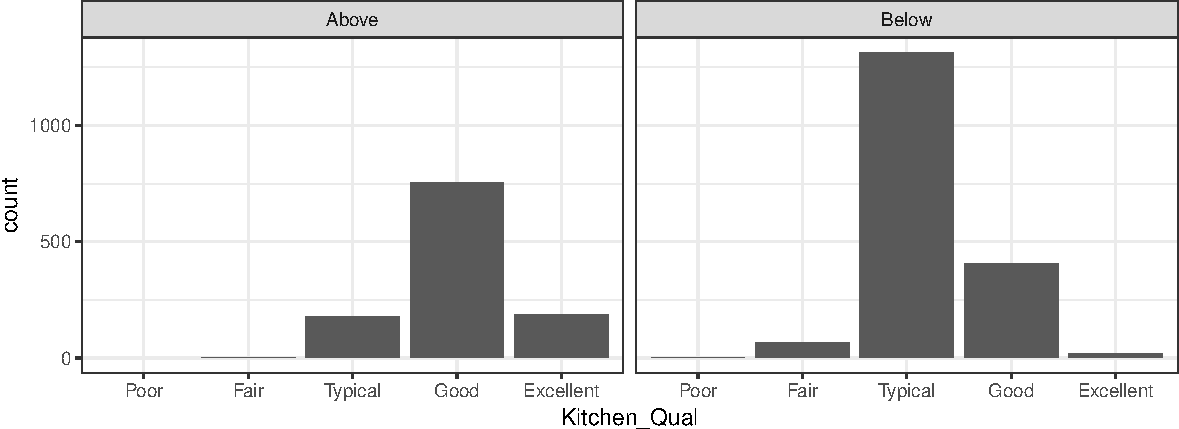
\includegraphics{Chapter_3_-_Visualization_files/figure-latex/facetw_bar-1} \end{center}

We can build onto this with \texttt{facet\_grid} which allows us to
create small multiples across two additional dimensions. In this example
we assess the quality of kitchens for homes that sold above and below
the mean sales price by neighborhood. This plot allows us to see gaps
across the different categorical levels along with which category
combinations are most frequent.

\begin{Shaded}
\begin{Highlighting}[]
\NormalTok{ames }\OperatorTok
\StringTok{  }\KeywordTok{mutate}\NormalTok{(}
    \DataTypeTok{Above_Avg =} \KeywordTok{ifelse}\NormalTok{(Sale_Price }\OperatorTok{>}\StringTok{ }\KeywordTok{mean}\NormalTok{(Sale_Price), }\StringTok{"Above"}\NormalTok{, }\StringTok{"Below"}\NormalTok{),}
    \DataTypeTok{Kitchen_Qual =} \KeywordTok{fct_relevel}\NormalTok{(Kitchen_Qual, }\StringTok{"Poor"}\NormalTok{, }\StringTok{"Fair"}\NormalTok{, }\StringTok{"Typical"}\NormalTok{, }\StringTok{"Good"}\NormalTok{)}
\NormalTok{    ) }\OperatorTok
\StringTok{  }\KeywordTok{group_by}\NormalTok{(Neighborhood, Above_Avg, Kitchen_Qual) }\OperatorTok
\StringTok{  }\KeywordTok{tally}\NormalTok{() }\OperatorTok
\StringTok{  }\KeywordTok{mutate}\NormalTok{(}\DataTypeTok{pct =}\NormalTok{ n }\OperatorTok{/}\StringTok{ }\KeywordTok{sum}\NormalTok{(n)) }\OperatorTok
\StringTok{  }\KeywordTok{ggplot}\NormalTok{(}\KeywordTok{aes}\NormalTok{(Kitchen_Qual, pct)) }\OperatorTok{+}\StringTok{ }
\StringTok{  }\KeywordTok{geom_col}\NormalTok{() }\OperatorTok{+}
\StringTok{  }\KeywordTok{facet_grid}\NormalTok{(Neighborhood }\OperatorTok{~}\StringTok{ }\NormalTok{Above_Avg) }\OperatorTok{+}
\StringTok{  }\KeywordTok{theme}\NormalTok{(}\DataTypeTok{strip.text.y =} \KeywordTok{element_text}\NormalTok{(}\DataTypeTok{angle =} \DecValTok{0}\NormalTok{, }\DataTypeTok{hjust =} \DecValTok{0}\NormalTok{))}
\end{Highlighting}
\end{Shaded}

\begin{center}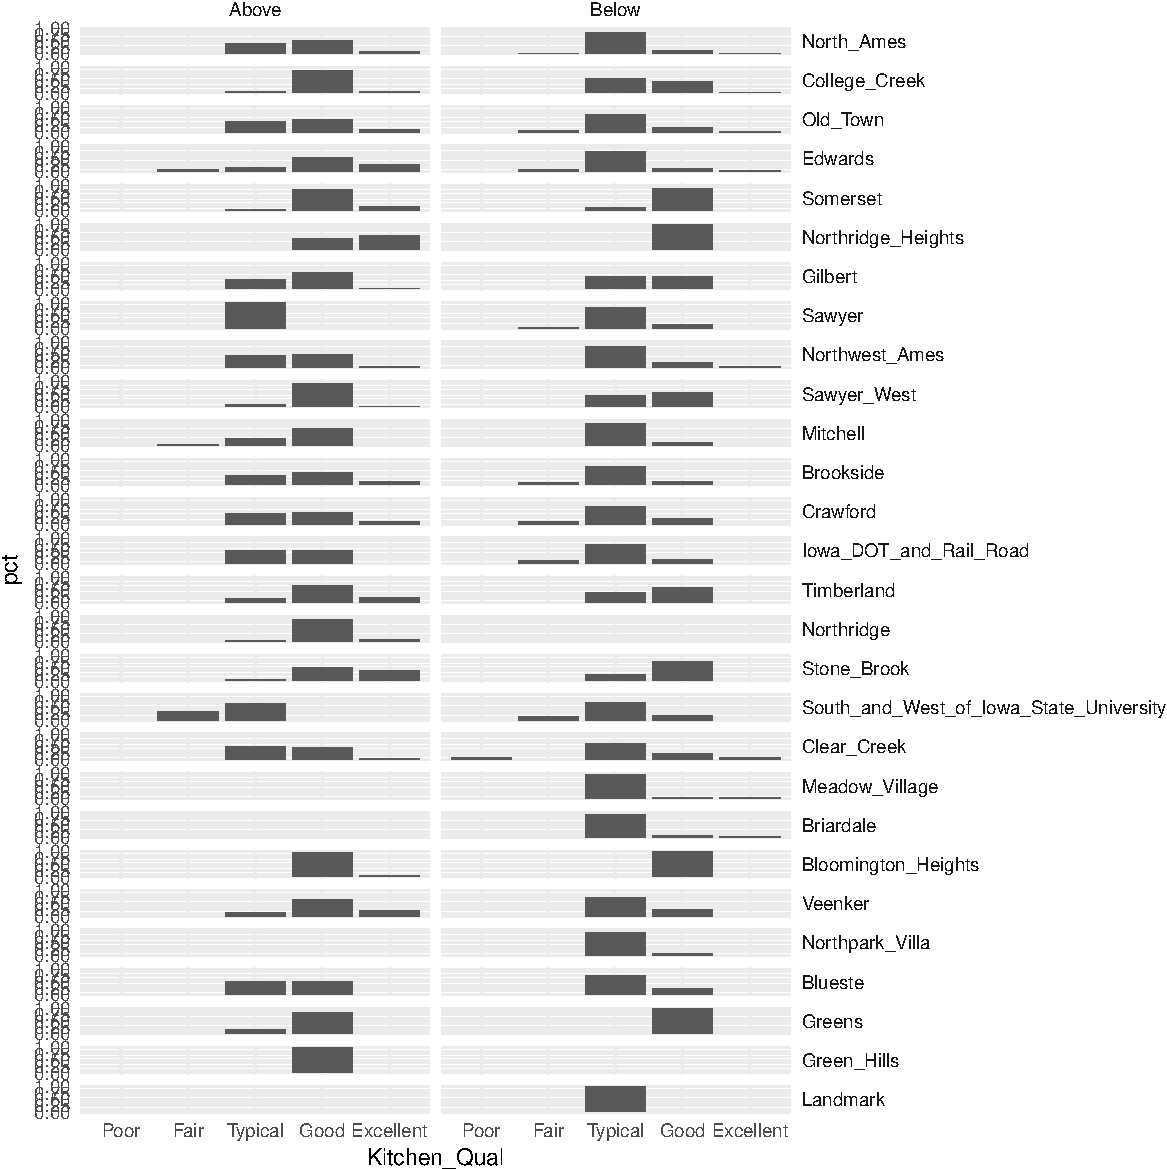
\includegraphics{Chapter_3_-_Visualization_files/figure-latex/facetg_bar-1} \end{center}

\section{Multivariate Relationships}\label{multivariate-relationships}

In most analyses, data are usually multivariate by nature, and the
analytics are designed to capture and measure multivariate
relationships. Visual exploration should therefore also incorporate this
important aspect. We can extend these basic principles and add in
additional features to assess multidimensional relationships. One
approach is to add additional variables with features such as color,
shape, or size. For example, here we compare the sales price to above
ground square footage of homes with and without central air
conditioning. We can see that there are far more homes with central air
and that those homes without central air tend to have less square
footage and sell for lower sales prices.

\begin{Shaded}
\begin{Highlighting}[]
\KeywordTok{ggplot}\NormalTok{(ames, }\KeywordTok{aes}\NormalTok{(}\DataTypeTok{x =}\NormalTok{ Gr_Liv_Area, }\DataTypeTok{y =}\NormalTok{ Sale_Price, }\DataTypeTok{color =}\NormalTok{ Central_Air, }\DataTypeTok{shape =}\NormalTok{ Central_Air)) }\OperatorTok{+}
\StringTok{  }\KeywordTok{geom_point}\NormalTok{(}\DataTypeTok{alpha =}\NormalTok{ .}\DecValTok{3}\NormalTok{) }\OperatorTok{+}
\StringTok{  }\KeywordTok{scale_x_log10}\NormalTok{() }\OperatorTok{+}
\StringTok{  }\KeywordTok{scale_y_log10}\NormalTok{()}
\end{Highlighting}
\end{Shaded}

\begin{center}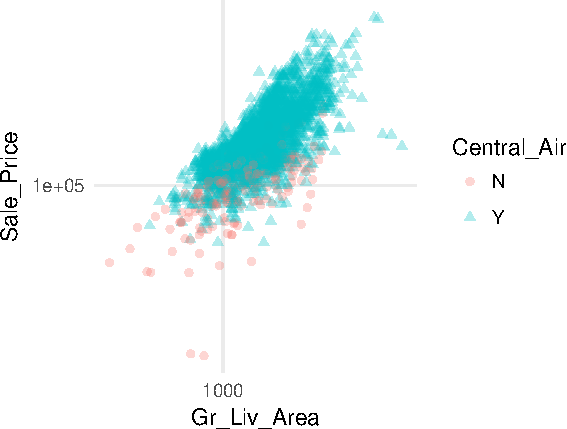
\includegraphics{Chapter_3_-_Visualization_files/figure-latex/multidim1-1} \end{center}

However, as before, when there are many levels in a categorical variable
it becomes hard to compare differences by only incorporating color or
shape features. An alternative is to create small multiples. Here we
compare the relationship between sales price and above ground square
footage and we assess how this relationship may differ across the
different house styles (i.e.~one story, two story, etc.).

\begin{Shaded}
\begin{Highlighting}[]
\KeywordTok{ggplot}\NormalTok{(ames, }\KeywordTok{aes}\NormalTok{(}\DataTypeTok{x =}\NormalTok{ Gr_Liv_Area, }\DataTypeTok{y =}\NormalTok{ Sale_Price)) }\OperatorTok{+}
\StringTok{  }\KeywordTok{geom_point}\NormalTok{(}\DataTypeTok{alpha =}\NormalTok{ .}\DecValTok{3}\NormalTok{) }\OperatorTok{+}
\StringTok{  }\KeywordTok{scale_x_log10}\NormalTok{() }\OperatorTok{+}
\StringTok{  }\KeywordTok{scale_y_log10}\NormalTok{(}\DataTypeTok{labels =}\NormalTok{ scales}\OperatorTok{::}\NormalTok{dollar) }\OperatorTok{+}
\StringTok{  }\KeywordTok{facet_wrap}\NormalTok{(}\OperatorTok{~}\StringTok{ }\NormalTok{House_Style, }\DataTypeTok{nrow =} \DecValTok{2}\NormalTok{) }\OperatorTok{+}
\StringTok{  }\KeywordTok{theme_bw}\NormalTok{()}
\end{Highlighting}
\end{Shaded}

\begin{center}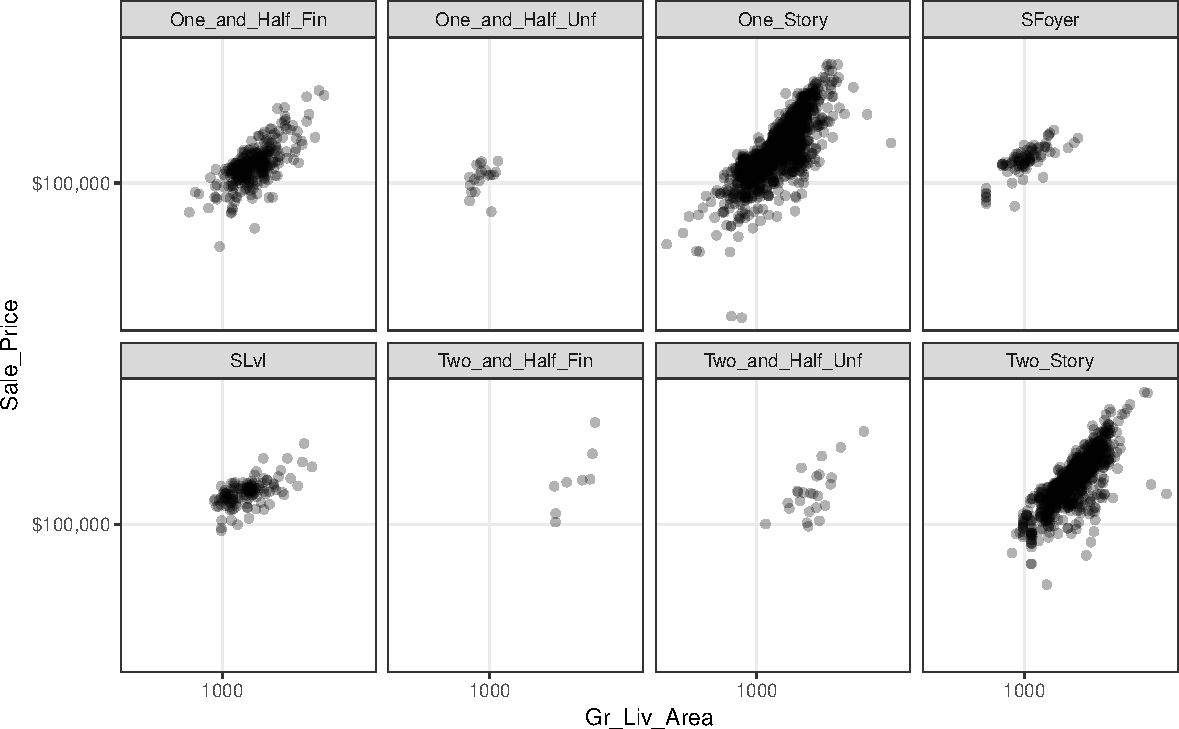
\includegraphics{Chapter_3_-_Visualization_files/figure-latex/smallmulti-1} \end{center}

We can start to add several of the features discussed in this chapter to
highlight mutlivariate features. For example, here we assess the
relationship between sales price and above ground square footage for
homes with and without central air conditioning and across the different
housing styles. For each house style and central air category we can see
where the values are clustered and how the linear relationship changes.
For all home styles, houses with central air have a higher selling price
with a steeper slope than those without central air. Also, those plots
without density markings and linear lines for the no central air
category (red) tell us that there are no more than one observation in
these groups; so this identifies gaps across multivariate categories of
interest.

\begin{Shaded}
\begin{Highlighting}[]
\KeywordTok{ggplot}\NormalTok{(ames, }\KeywordTok{aes}\NormalTok{(}\DataTypeTok{x =}\NormalTok{ Gr_Liv_Area, }\DataTypeTok{y =}\NormalTok{ Sale_Price, }\DataTypeTok{color =}\NormalTok{ Central_Air, }\DataTypeTok{shape =}\NormalTok{ Central_Air)) }\OperatorTok{+}
\StringTok{  }\KeywordTok{geom_point}\NormalTok{(}\DataTypeTok{alpha =}\NormalTok{ .}\DecValTok{3}\NormalTok{) }\OperatorTok{+}
\StringTok{  }\KeywordTok{geom_density2d}\NormalTok{(}\DataTypeTok{alpha =}\NormalTok{ .}\DecValTok{5}\NormalTok{) }\OperatorTok{+}
\StringTok{  }\KeywordTok{geom_smooth}\NormalTok{(}\DataTypeTok{method =} \StringTok{"lm"}\NormalTok{, }\DataTypeTok{se =} \OtherTok{FALSE}\NormalTok{) }\OperatorTok{+}
\StringTok{  }\KeywordTok{scale_x_log10}\NormalTok{() }\OperatorTok{+}
\StringTok{  }\KeywordTok{scale_y_log10}\NormalTok{(}\DataTypeTok{labels =}\NormalTok{ scales}\OperatorTok{::}\NormalTok{dollar) }\OperatorTok{+}
\StringTok{  }\KeywordTok{facet_wrap}\NormalTok{(}\OperatorTok{~}\StringTok{ }\NormalTok{House_Style, }\DataTypeTok{nrow =} \DecValTok{2}\NormalTok{) }\OperatorTok{+}
\StringTok{  }\KeywordTok{ggtitle}\NormalTok{(}\StringTok{"Sale Price vs. Above Ground Sq.Ft"}\NormalTok{,}
          \DataTypeTok{subtitle =} \StringTok{"How does central air and house style influence this relationship?"}\NormalTok{) }\OperatorTok{+}
\StringTok{  }\KeywordTok{theme_bw}\NormalTok{()}
\end{Highlighting}
\end{Shaded}

\begin{center}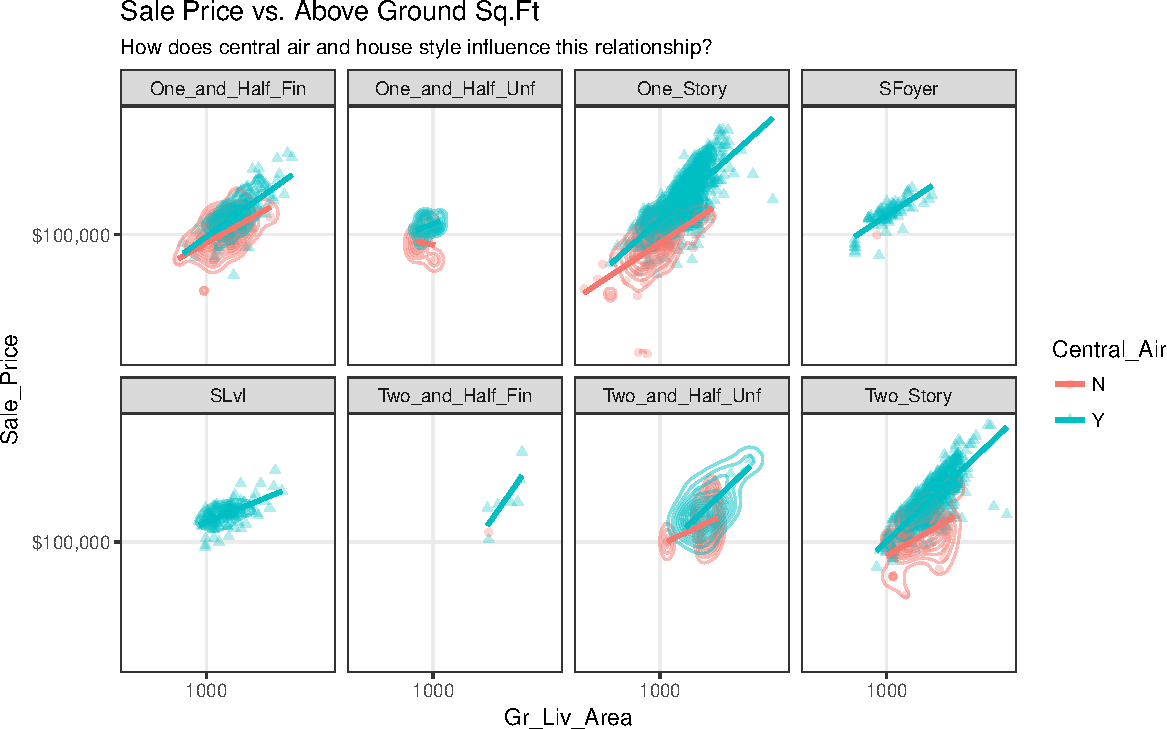
\includegraphics{Chapter_3_-_Visualization_files/figure-latex/multivar1-1} \end{center}

Parallel coordinate plots (PCP) are also a great way to visualize
continuous variables across multiple variables. In these plots, a
vertical axis is drawn for each variable. Then each observation is
represented by drawing a line that connects its values on the different
axes, thereby creating a multivariate profile. To create a PCP, we can
use \texttt{ggparcoord} from the \texttt{GGally} package. By default,
\texttt{ggparcoord} will standardize the variables based on a Z-score
distribution; however, there are many options for scaling (see
\texttt{?ggparcoord}). One benefit of of a PCP is that you can visualize
your observations across continuous and categorical variables. In this
example I include \texttt{Overall\_Qual} which is an ordered factor with
levels ``Very Poor'', ``Poor'', ``Fair'', \ldots{}, ``Excellent'',
``Very Excellent'' having values of 1-10. When including a factor
variable \texttt{ggparcoord} will use the factor integer levels for
their value so it is important to appropriately order any factors you
want to include.

\begin{Shaded}
\begin{Highlighting}[]
\NormalTok{variables <-}\StringTok{ }\KeywordTok{c}\NormalTok{(}\StringTok{"Sale_Price"}\NormalTok{, }\StringTok{"Year_Built"}\NormalTok{, }\StringTok{"Year_Remod_Add"}\NormalTok{, }\StringTok{"Overall_Qual"}\NormalTok{)}

\NormalTok{ames }\OperatorTok
\StringTok{  }\KeywordTok{select}\NormalTok{(variables) }\OperatorTok
\StringTok{  }\KeywordTok{ggparcoord}\NormalTok{(}\DataTypeTok{alpha =}\NormalTok{ .}\DecValTok{05}\NormalTok{, }\DataTypeTok{scale =} \StringTok{"center"}\NormalTok{)}
\end{Highlighting}
\end{Shaded}

\begin{center}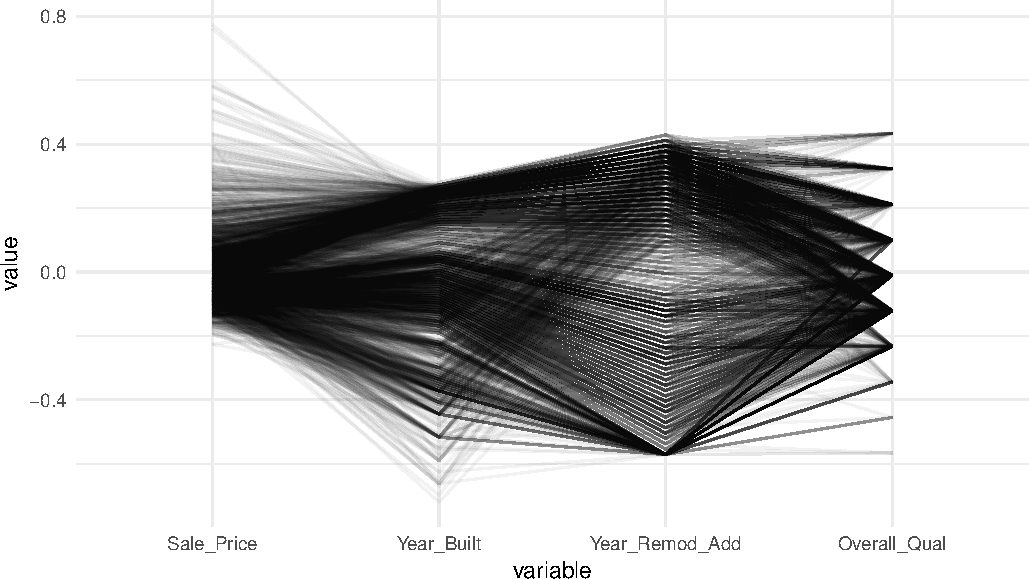
\includegraphics{Chapter_3_-_Visualization_files/figure-latex/parallel1-1} \end{center}

The darker bands in the above plot illustrate several features. The
observations with higher sales prices tend to be built in more recent
years, be remodeled in recent years and be categorized in the top half
of the overall quality measures. In contracts, homes with lower sales
prices tend to be more out-dated (based on older built and remodel
dates) and have lower quality ratings. We also see some homes with
exceptionally old build dates that have much newer remodel dates but
still have just average quality ratings.

We can make this more explicit by adding a new variable to indicate if a
sale price is above average. We can then tell \texttt{ggparcood} to
group by this new variable. Now we clearly see that above average sale
prices are related to much newer homes.

\begin{Shaded}
\begin{Highlighting}[]
\NormalTok{ames }\OperatorTok
\StringTok{  }\KeywordTok{select}\NormalTok{(variables) }\OperatorTok
\StringTok{  }\KeywordTok{mutate}\NormalTok{(}\DataTypeTok{Above_Avg =}\NormalTok{ Sale_Price }\OperatorTok{>}\StringTok{ }\KeywordTok{mean}\NormalTok{(Sale_Price)) }\OperatorTok
\StringTok{  }\KeywordTok{ggparcoord}\NormalTok{(}
    \DataTypeTok{alpha =}\NormalTok{ .}\DecValTok{05}\NormalTok{,}
    \DataTypeTok{scale =} \StringTok{"center"}\NormalTok{,}
    \DataTypeTok{columns =} \DecValTok{1}\OperatorTok{:}\DecValTok{4}\NormalTok{,}
    \DataTypeTok{groupColumn =} \StringTok{"Above_Avg"}
\NormalTok{    )}
\end{Highlighting}
\end{Shaded}

\begin{center}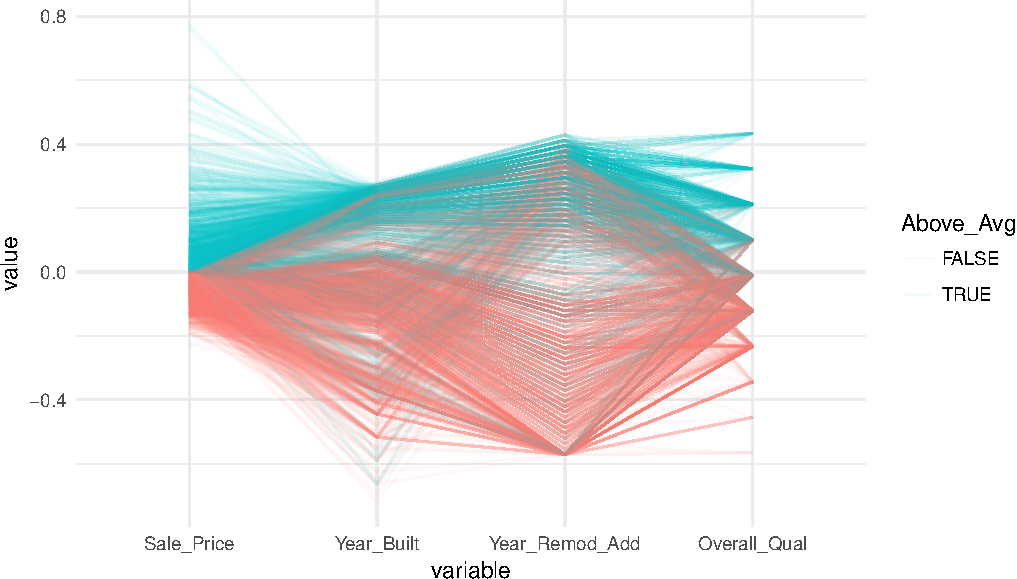
\includegraphics{Chapter_3_-_Visualization_files/figure-latex/parallel2-1} \end{center}

Mosaic plots are a graphical method for visualizing data from two or
more qualitative variables. In this visual the graphics area is divided
up into rectangles proportional in size to the counts of the
combinations they represent.

\begin{Shaded}
\begin{Highlighting}[]
\NormalTok{ames2 <-}\StringTok{ }\NormalTok{ames }\OperatorTok
\StringTok{  }\KeywordTok{mutate}\NormalTok{(}
    \DataTypeTok{Above_Avg =}\NormalTok{ Sale_Price }\OperatorTok{>}\StringTok{ }\KeywordTok{mean}\NormalTok{(Sale_Price),}
    \DataTypeTok{Garage_Type =} \KeywordTok{abbreviate}\NormalTok{(Garage_Type),}
    \DataTypeTok{Garage_Qual =} \KeywordTok{abbreviate}\NormalTok{(Garage_Qual)}
\NormalTok{         )}

\KeywordTok{par}\NormalTok{(}\DataTypeTok{mfrow =} \KeywordTok{c}\NormalTok{(}\DecValTok{1}\NormalTok{, }\DecValTok{2}\NormalTok{))}
\KeywordTok{mosaicplot}\NormalTok{(Above_Avg }\OperatorTok{~}\StringTok{ }\NormalTok{Garage_Type, }\DataTypeTok{data =}\NormalTok{ ames2, }\DataTypeTok{las =} \DecValTok{1}\NormalTok{)}
\KeywordTok{mosaicplot}\NormalTok{(Above_Avg }\OperatorTok{~}\StringTok{ }\NormalTok{Garage_Type }\OperatorTok{+}\StringTok{ }\NormalTok{Garage_Cars, }\DataTypeTok{data =}\NormalTok{ ames2, }\DataTypeTok{las =} \DecValTok{1}\NormalTok{)}
\end{Highlighting}
\end{Shaded}

\begin{center}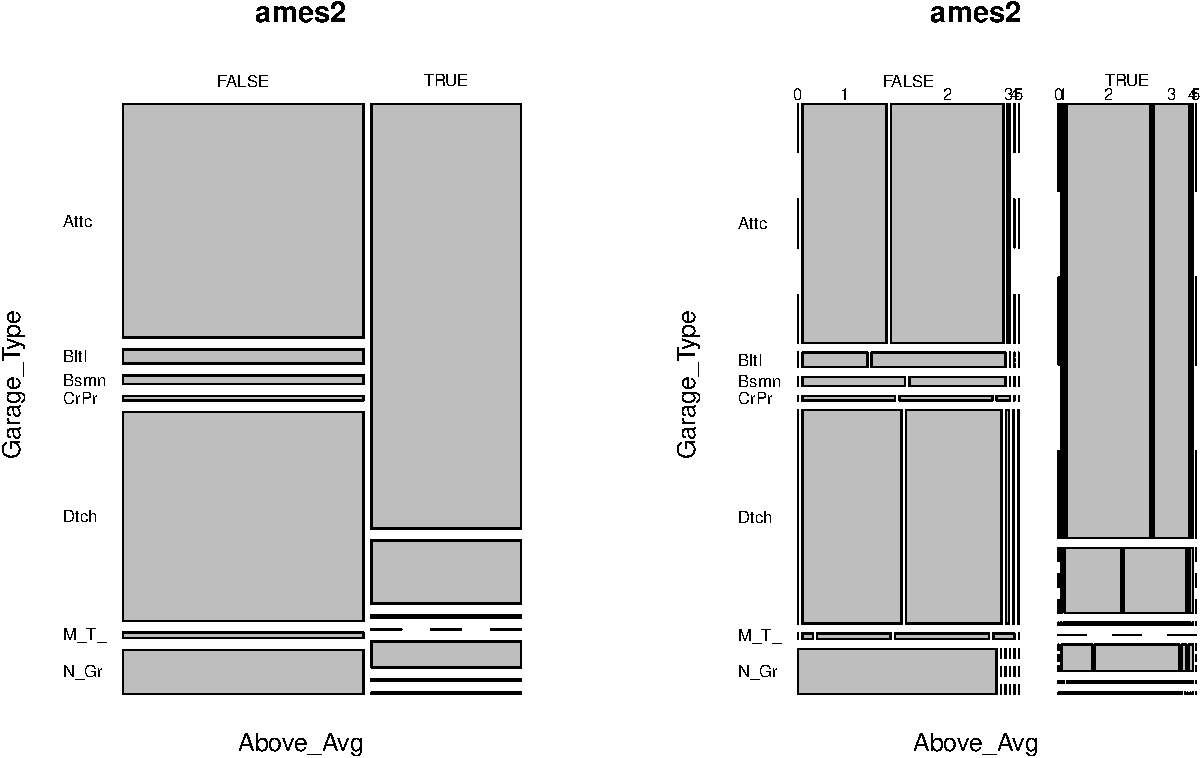
\includegraphics{Chapter_3_-_Visualization_files/figure-latex/mosaic-1} \end{center}

Treemaps are also a useful visualization aimed at assessing the
hierarchical structure of data. Treemaps are primarily used to assess a
numeric value across multiple categories. It can be useful to assess the
counts or porportions of a categorical variable nested within other
categorical variables. For example, we can use a treemap to visualize
the above right mosaic plot that illustrates the number of homes sold
above and below average sales price with different garage
characteristics. We can see in the treemap that houses with above
average prices tend to have attached 2 and 3-car garages. Houses sold
below average price have more attached 1-car garages and also have far
more detached garages.

\begin{Shaded}
\begin{Highlighting}[]
\NormalTok{ames }\OperatorTok\StringTok{ }
\StringTok{  }\KeywordTok{mutate}\NormalTok{(}\DataTypeTok{Above_Below =} \KeywordTok{ifelse}\NormalTok{(Sale_Price }\OperatorTok{>}\StringTok{ }\KeywordTok{mean}\NormalTok{(Sale_Price), }\StringTok{"Above Avg"}\NormalTok{, }\StringTok{"Below Avg"}\NormalTok{)) }\OperatorTok
\StringTok{  }\KeywordTok{count}\NormalTok{(Garage_Type, Garage_Cars, Above_Below) }\OperatorTok
\StringTok{  }\KeywordTok{treemap}\NormalTok{(}
    \DataTypeTok{index =} \KeywordTok{c}\NormalTok{(}\StringTok{"Above_Below"}\NormalTok{, }\StringTok{"Garage_Type"}\NormalTok{, }\StringTok{"Garage_Cars"}\NormalTok{),}
    \DataTypeTok{vSize =} \StringTok{"n"}
\NormalTok{  )}
\end{Highlighting}
\end{Shaded}

\begin{center}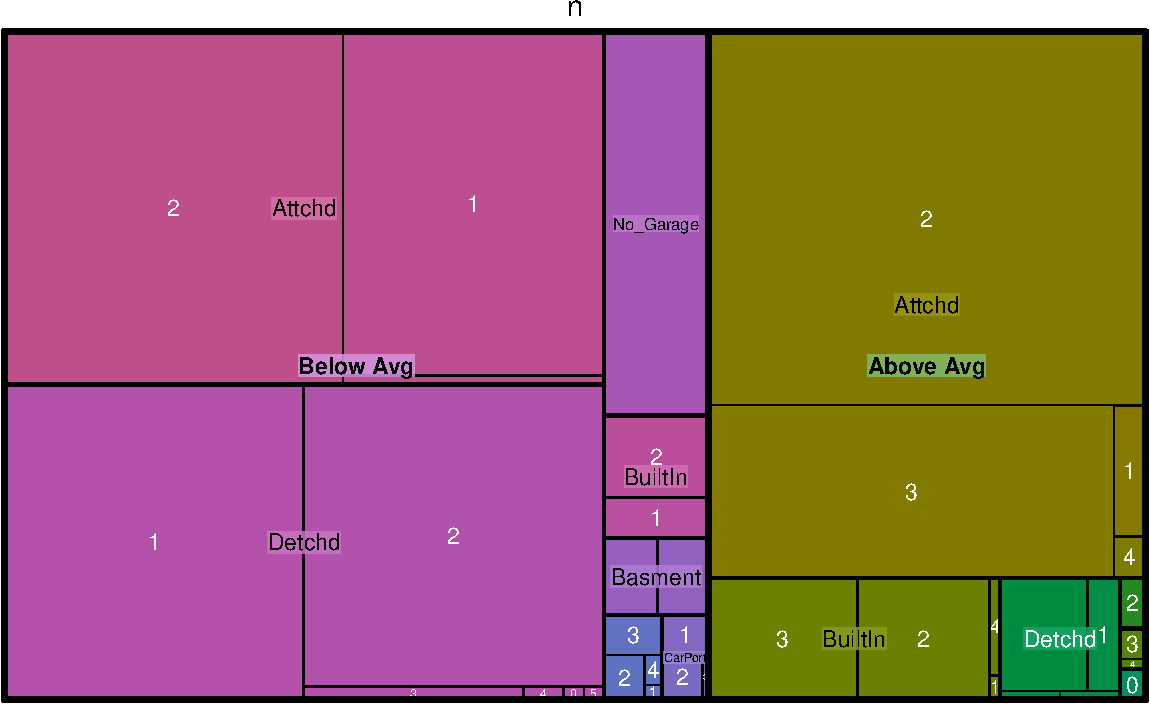
\includegraphics{Chapter_3_-_Visualization_files/figure-latex/mosaic2-1} \end{center}

A heatmap is a graphical display of numerical data where color is used
to denote the case value realtive to other values in the column.
Heatmaps can be extremely useful in identify clusters of strongly
correlated values. We can select all numeric variables in our
\texttt{ames} data set, compute the correlation matrix and visualize
this matrix with a heatmap. Those locations with dark red represent
correlations with smaller values while lighter colored cells represent
larger values. Looking at \texttt{Sale\_Price} (3rd row from top) you
can see that the smaller values are clustered to the left of the plot
suggestion weaker linear relationships with variables such as
\texttt{BsmtFin\_Sf\_1}, \texttt{Bsmt\_Unf\_SF}, \texttt{Longitude},
\texttt{Enclosed\_Porch}, etc. The larger correlations values for
\texttt{Sale\_Price} align with variables to the right of the plot such
as \texttt{Garage\_Cars}, \texttt{Garage\_Area},
\texttt{First\_Flr\_SF}, etc.

\begin{Shaded}
\begin{Highlighting}[]
\NormalTok{ames }\OperatorTok
\StringTok{  }\KeywordTok{select_if}\NormalTok{(is.numeric) }\OperatorTok
\StringTok{  }\KeywordTok{cor}\NormalTok{() }\OperatorTok
\StringTok{  }\KeywordTok{heatmap}\NormalTok{()}
\end{Highlighting}
\end{Shaded}

\begin{center}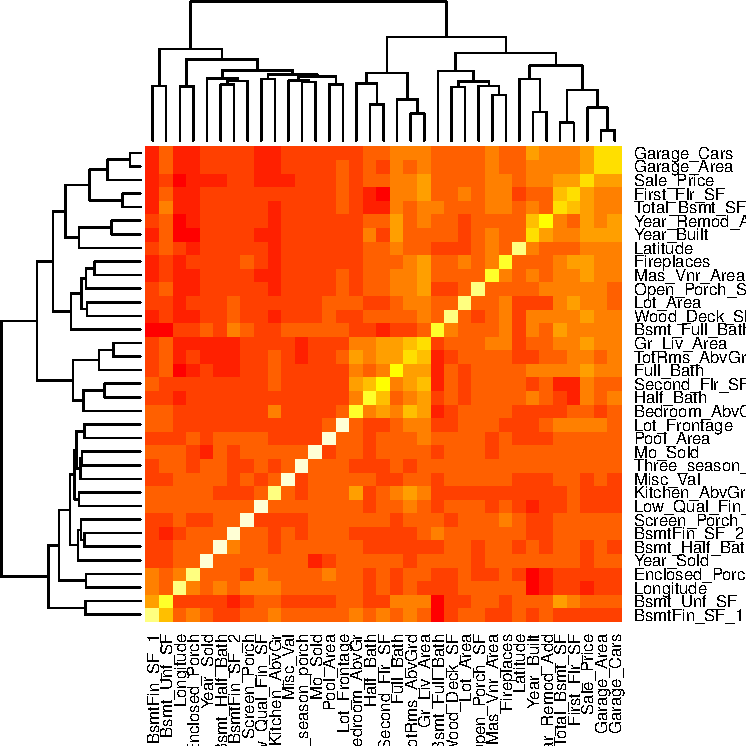
\includegraphics{Chapter_3_-_Visualization_files/figure-latex/heatmap-1} \end{center}

A heatmap is a great way to assess the relationship across a large data
set. However, when you are dealing with a smaller data set (or subset),
you may want to create a matrix plot to compare relationships across all
variables. For example, here I select \texttt{Sale\_Price} and all
variables that contain ``sf'' (all square footage variables), I scale
all variables, and then visualize the scatter plot and correlation
values with \texttt{GGally::ggpairs}.

\begin{Shaded}
\begin{Highlighting}[]
\NormalTok{ames }\OperatorTok
\StringTok{  }\KeywordTok{select}\NormalTok{(Sale_Price, }\KeywordTok{contains}\NormalTok{(}\StringTok{"sf"}\NormalTok{)) }\OperatorTok
\StringTok{  }\KeywordTok{map_df}\NormalTok{(scale) }\OperatorTok
\StringTok{  }\KeywordTok{ggpairs}\NormalTok{()}
\end{Highlighting}
\end{Shaded}

\begin{center}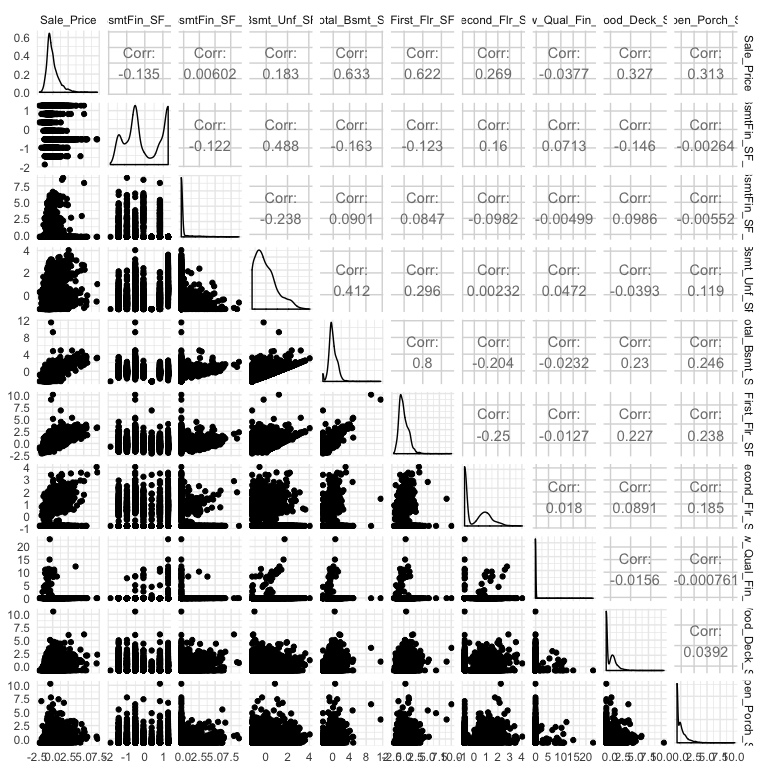
\includegraphics{Chapter_3_-_Visualization_files/figure-latex/ggpairs-1} \end{center}

\section{Data Quality}\label{data-quality}

Graphical displays can also assist in summarizing certain data quality
features. In the previous sections we illustrated how we can identify
outliers but missing data also represent an important characteristic of
our data. This chapter has been using the processed version of the Ames
housing data set. However, if we use the raw data we see that there are
13,997 missing values. It is important to understand how these missing
values are dispersed acrossed a data set as that can determine if you
need to eliminate a variable or if you can impute.

\begin{Shaded}
\begin{Highlighting}[]
\KeywordTok{sum}\NormalTok{(}\KeywordTok{is.na}\NormalTok{(AmesHousing}\OperatorTok{::}\NormalTok{ames_raw))}
\NormalTok{## [1] 13997}
\end{Highlighting}
\end{Shaded}

Heatmaps have a nice alternative use case for visualizing missing values
across a data set. In this example
\texttt{is.na(AmesHousing::ames\_raw)} will return a Boolean
(TRUE/FALSE) output indicating the location of missing values and by
multiplying this value by 1 converts the output to 0/1 binary to be
plotted. All yellow locations in our heatmap represent missing values.
This allows us to see those variables where the majority of the
observations have missing values (i.e. \texttt{Alley},
\texttt{Fireplace\ Qual}, \texttt{Pool\ QC}, \texttt{Fence}, and
\texttt{Misc\ Feature}). Due to their high frequency of missingness,
these variables would likely need to be removed from future analytic
approaches. However, we can also spot other unique features of
missingness. For example, missing values appear to occur across all
garage variables for the same observations.

\begin{Shaded}
\begin{Highlighting}[]
\KeywordTok{heatmap}\NormalTok{(}\DecValTok{1} \OperatorTok{*}\StringTok{ }\KeywordTok{is.na}\NormalTok{(AmesHousing}\OperatorTok{::}\NormalTok{ames_raw), }\DataTypeTok{Rowv =} \OtherTok{NA}\NormalTok{, }\DataTypeTok{Colv =} \OtherTok{NA}\NormalTok{)}
\end{Highlighting}
\end{Shaded}

\begin{center}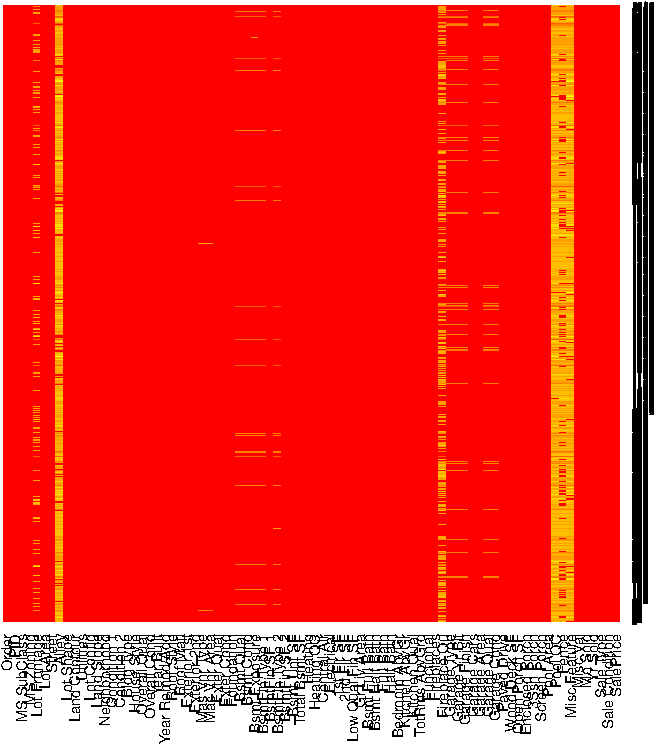
\includegraphics{Chapter_3_-_Visualization_files/figure-latex/heatmap2-1} \end{center}

If we dig a little deeper into these variables we would notice that
\texttt{Garage\ Cars} and \texttt{Garage\ Area} all contain the value 0
for every observation where the other \texttt{Garage\_xx} variables have
missing values. This is because in the raw Ames housing data set, they
did not have an option to identify houses with no garages. Therefore,
all houses with no garage were identified by including nothing. This
would be opportunity to create a new categorical level (``None'') for
these garage variables.

\begin{Shaded}
\begin{Highlighting}[]
\NormalTok{AmesHousing}\OperatorTok{::}\NormalTok{ames_raw }\OperatorTok\StringTok{ }
\StringTok{  }\KeywordTok{filter}\NormalTok{(}\KeywordTok{is.na}\NormalTok{(}\StringTok{`}\DataTypeTok{Garage Type}\StringTok{`}\NormalTok{)) }\OperatorTok\StringTok{ }
\StringTok{  }\KeywordTok{select}\NormalTok{(}\KeywordTok{contains}\NormalTok{(}\StringTok{"garage"}\NormalTok{))}
\NormalTok{## # A tibble: 157 x 7}
\NormalTok{##    `Garage Type` `Garage Yr Blt` `Garage Finish` `Gara~ `Gara~ `Gar~ `Gar~}
\NormalTok{##    <chr>                   <int> <chr>            <int>  <int> <chr> <chr>}
\NormalTok{##  1 <NA>                       NA <NA>                 0      0 <NA>  <NA> }
\NormalTok{##  2 <NA>                       NA <NA>                 0      0 <NA>  <NA> }
\NormalTok{##  3 <NA>                       NA <NA>                 0      0 <NA>  <NA> }
\NormalTok{##  4 <NA>                       NA <NA>                 0      0 <NA>  <NA> }
\NormalTok{##  5 <NA>                       NA <NA>                 0      0 <NA>  <NA> }
\NormalTok{##  6 <NA>                       NA <NA>                 0      0 <NA>  <NA> }
\NormalTok{##  7 <NA>                       NA <NA>                 0      0 <NA>  <NA> }
\NormalTok{##  8 <NA>                       NA <NA>                 0      0 <NA>  <NA> }
\NormalTok{##  9 <NA>                       NA <NA>                 0      0 <NA>  <NA> }
\NormalTok{## 10 <NA>                       NA <NA>                 0      0 <NA>  <NA> }
\NormalTok{## # ... with 147 more rows}
\end{Highlighting}
\end{Shaded}

An alternative approach is to use \texttt{extracat::visna}, which allows
us to visualize missing patters. The columns represent the 82 variables
and the rows the missing patterns. The cells for the variables with
missing values in a pattern are drawn in blue. The variables and
patterns have been ordered by numbers of missings on both rows and
columns (\texttt{sort\ =\ "b"}). The bars beneath the columns show the
proporations of missings by variable and the bars on the right show the
relative frequencies of patterns.

\begin{Shaded}
\begin{Highlighting}[]
\NormalTok{extracat}\OperatorTok{::}\KeywordTok{visna}\NormalTok{(AmesHousing}\OperatorTok{::}\NormalTok{ames_raw, }\DataTypeTok{sort =} \StringTok{"b"}\NormalTok{)}
\end{Highlighting}
\end{Shaded}

\begin{center}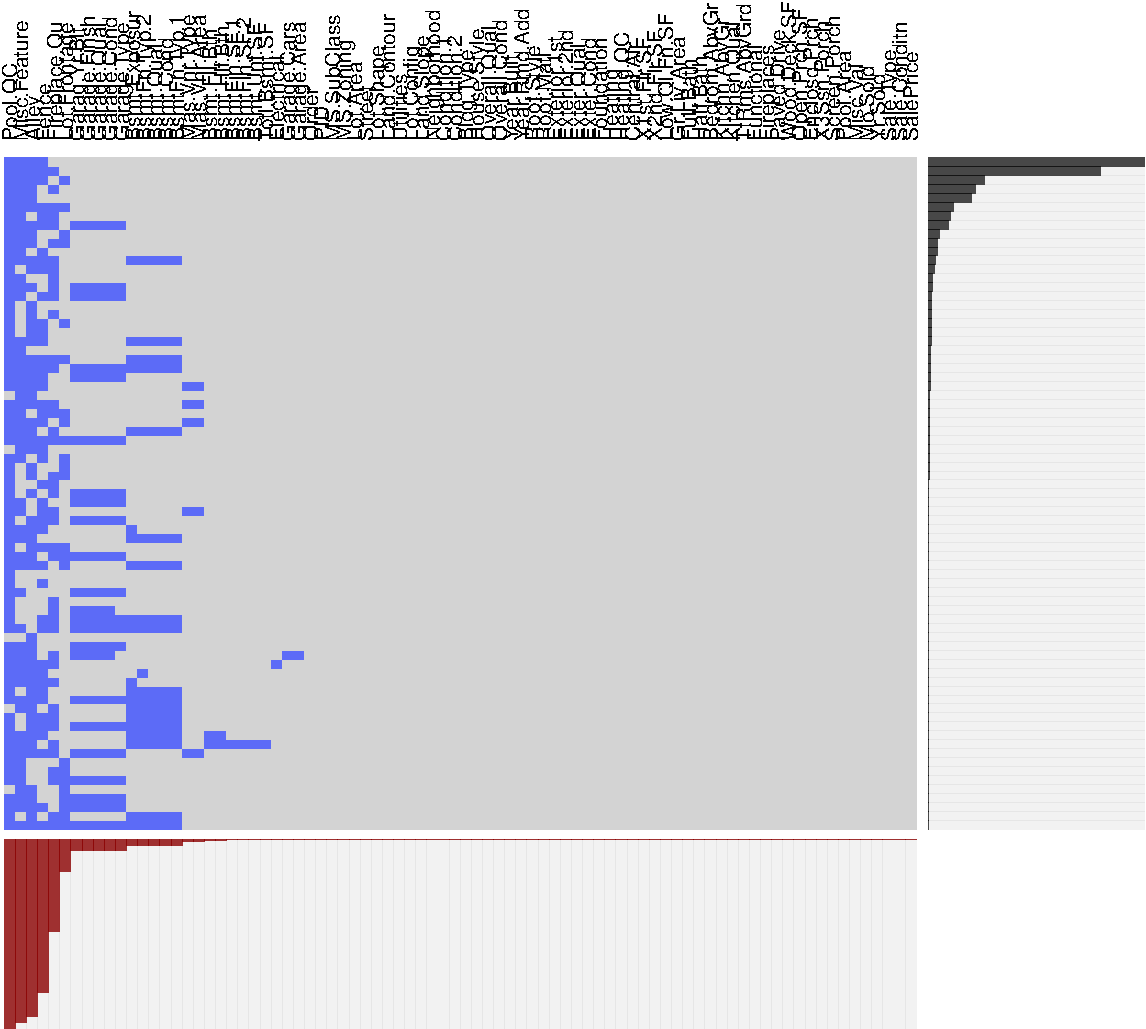
\includegraphics{Chapter_3_-_Visualization_files/figure-latex/missing2-1} \end{center}

Data can be missing for different reasons. It could be that a value was
not recorded, or that it was, but was obviously an error. As in our case
with the garage variables it could be because there was not an option to
record the specific value observed so the default action was to not
record any value. Regardless, it is important to identify and understand
how missing values are observed across a data set as they can provide
insight into how to deal with these observations.

\section{Exercises}\label{exercises}


\end{document}
